\chapter{Background}
\label{chapter:background} 

As outlined in the introduction, in this thesis we present a novel method for the projection mapping of textures. Our method follows a different goal than conventional projection mapping algorithms -- instead of the matching camera image with the desired appearance pixel by pixel, we force the camera image and the desired appearance to be realizations of the same texture (see eq. \ref{eq:projection_mapping-statistics}). This gives us more flexibility and enables us to bypass some restrictions imposed on the camera image by the scene and projector hardware.

We do not build our method from scratch, however. Many necessary building blocks have been introduced by other researchers in various fields. In this section, we present the work we build on and explain all concepts that lie behind our approach. Specifically, at the core of this chapter are the answers to the following questions:

\begin{itemize}
    \item How can we predict what an image will look like when projected onto a scene?
    \item Given a texture, how can we generate new realizations of it?
\end{itemize}

The former question is part of the field of projection mapping, while the latter represents the field of texture synthesis.

\section{Projection Mapping}
\label{section:background-projection_mapping}

In order to predict projection appearance, we first need to understand how projectors work, get an intuition of what to roughly expect when projecting on various surfaces and then understand the theory behind light transport. Finally, we can combine these concepts and study projector-camera systems and how they can help us answer our question.

\subsection{Projectors}
\label{section:background-projection_mapping-projectors}

Projectors are devices that transfer images onto surfaces such as screens, walls and other physical objects. The more traditional kind of projectors are film projectors, that shine a bright light through a film and a set of lenses. Nowadays, digital projectors are more common, but the core principle of shining a bright light through a device is still the same.

\begin{figure}[ht]
    \centering
    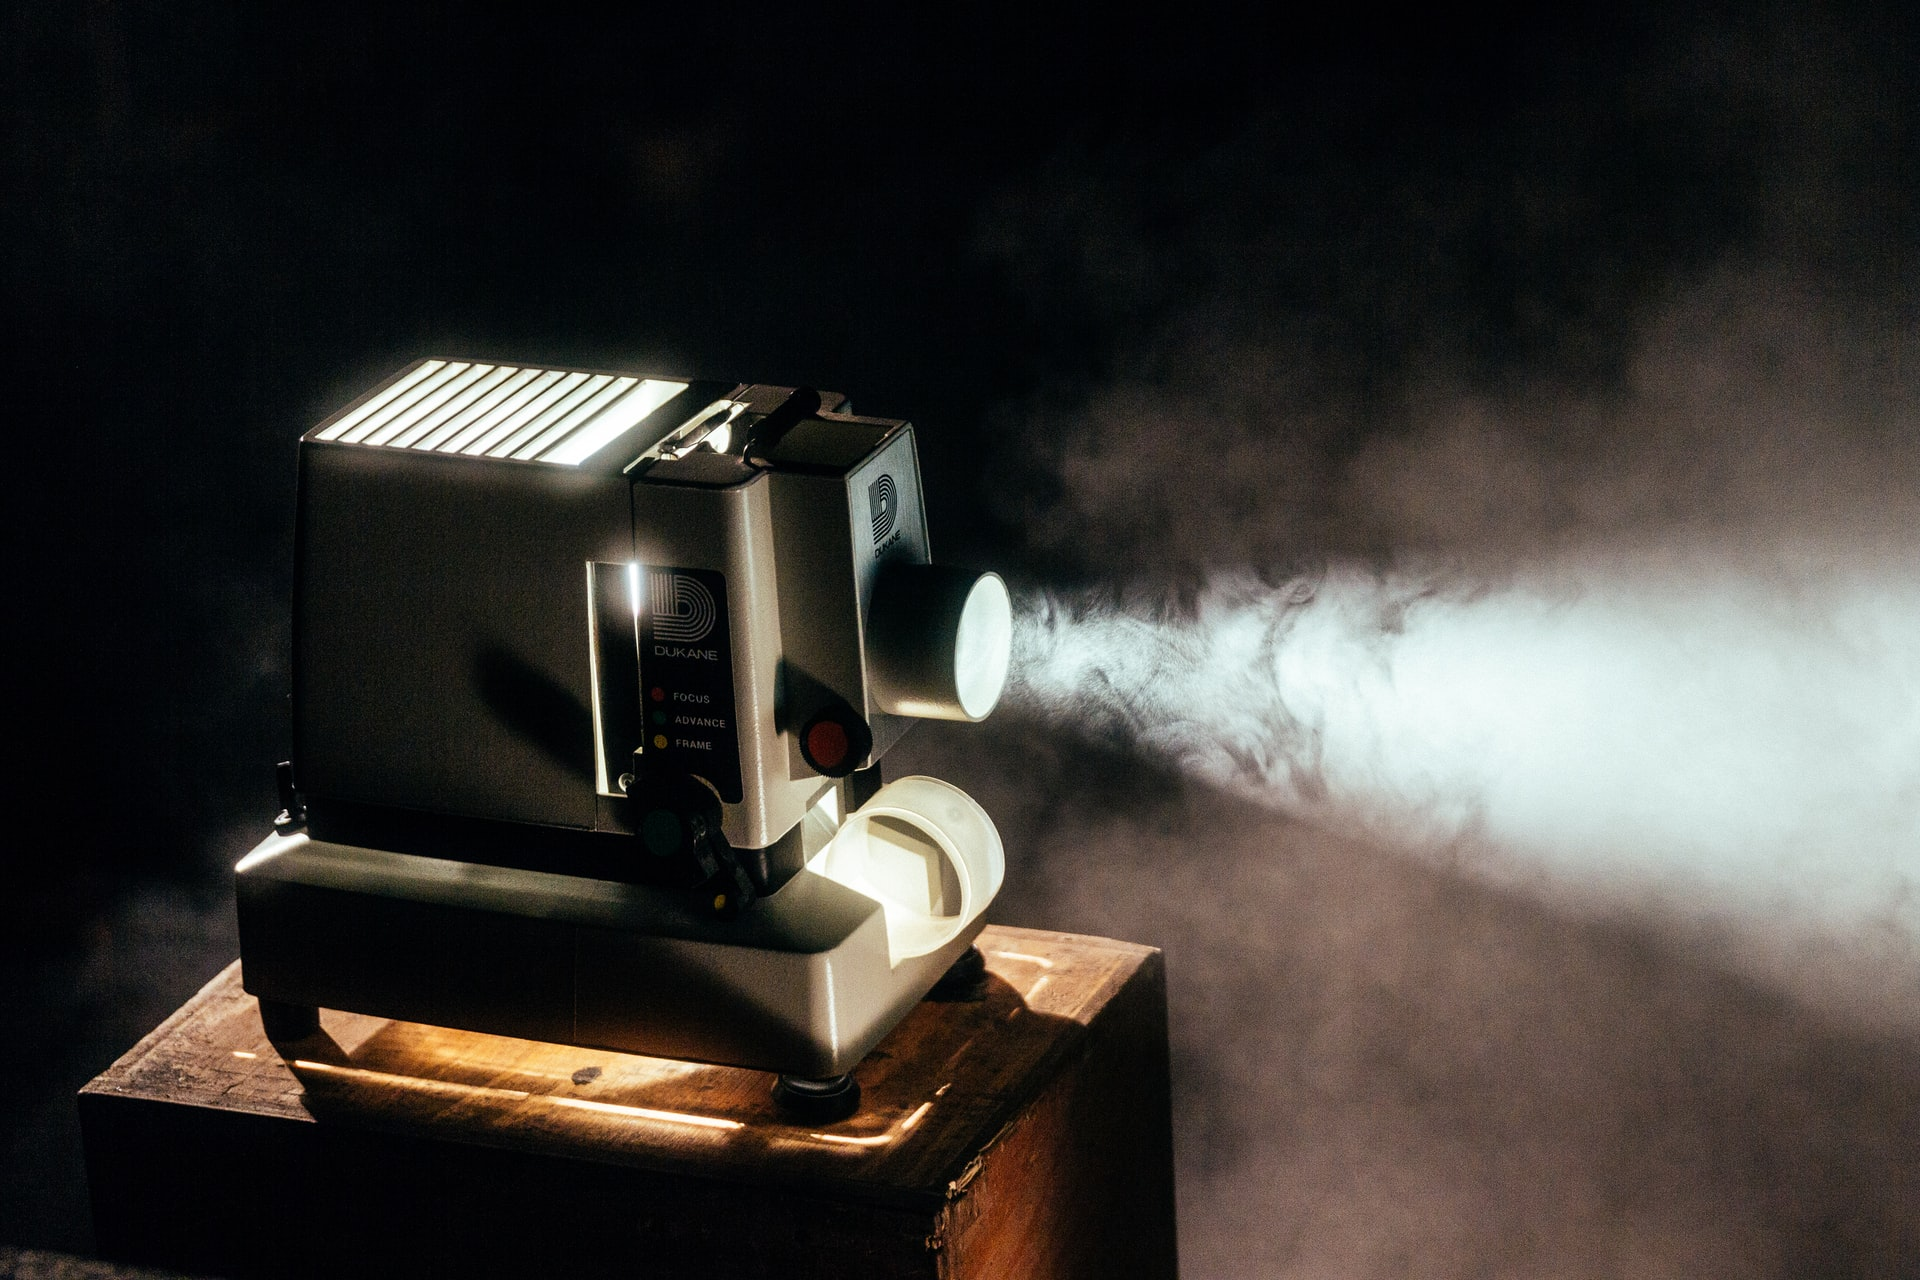
\includegraphics[width=0.8\textwidth]{images/02-projector.jpg}
    \caption{A projector is above all a light emitter. Source: \citet{ImageProjector}}
    \label{fig:background_projector}
\end{figure}

As briefly mentioned in section \ref{section:intro-problem_setting}, no projector is capable of reproducing arbitrary appearance. Each projector can only reproduce a subset of all possible colors, called the \textit{gamut}. Limited projector gamuts have a large impact on how projection mapping is done. To get a better intuition of this impact, we will now explain how a particular type of projector works. We will focus on the so-called Digital Light Processing (DLP) projector which is widely used in cinemas as well as home setups.

\subsubsection{DLP Projectors}
\label{section:background-projection_mapping-projectors-DLP}

Film projectors shine a bright light through film to project its contents onto a screen. But what happens when our movie is digital? What does a DLP projector shine its light through? And what impact does it have on its gamut?

According to \citet{WikiDLP}, DLP projectors project images by filtering the bright white light of their lamp. First, the light goes through a rapidly spinning color wheel which is split into a number of sectors: red, green, blue and sometimes also transparent. At any point, all light from the lamp passes through a single color filter, sending a single-channel image towards the lens. By sending out many single-channel images in rapid succession, however, the projector creates the illusion of sending a three-channel image.

Per-pixel intesities of this single-channel image which form its content are controlled by the Digital Micromirror Device (DMD). This device is divided into many tiny mirrors which roughly correspond to individual pixels of the projected image. Each of these mirrors can either reflect light from the color wheel directly into the lens, or into a heat sink which absorbs it and does not let it through. This allows the projector to turn pixels off and on. Grayscales (pixel intensities between full and zero) are produced by rapidly toggling the mirror between the lens and the heat sink. If, for example, a pixel is on 50\% of the time and off 50\% of the time, the resulting intensity is exactly between full and zero.

\begin{figure}[ht]
    \centering
    \begin{subfigure}[b]{0.49\textwidth}
        \centering
        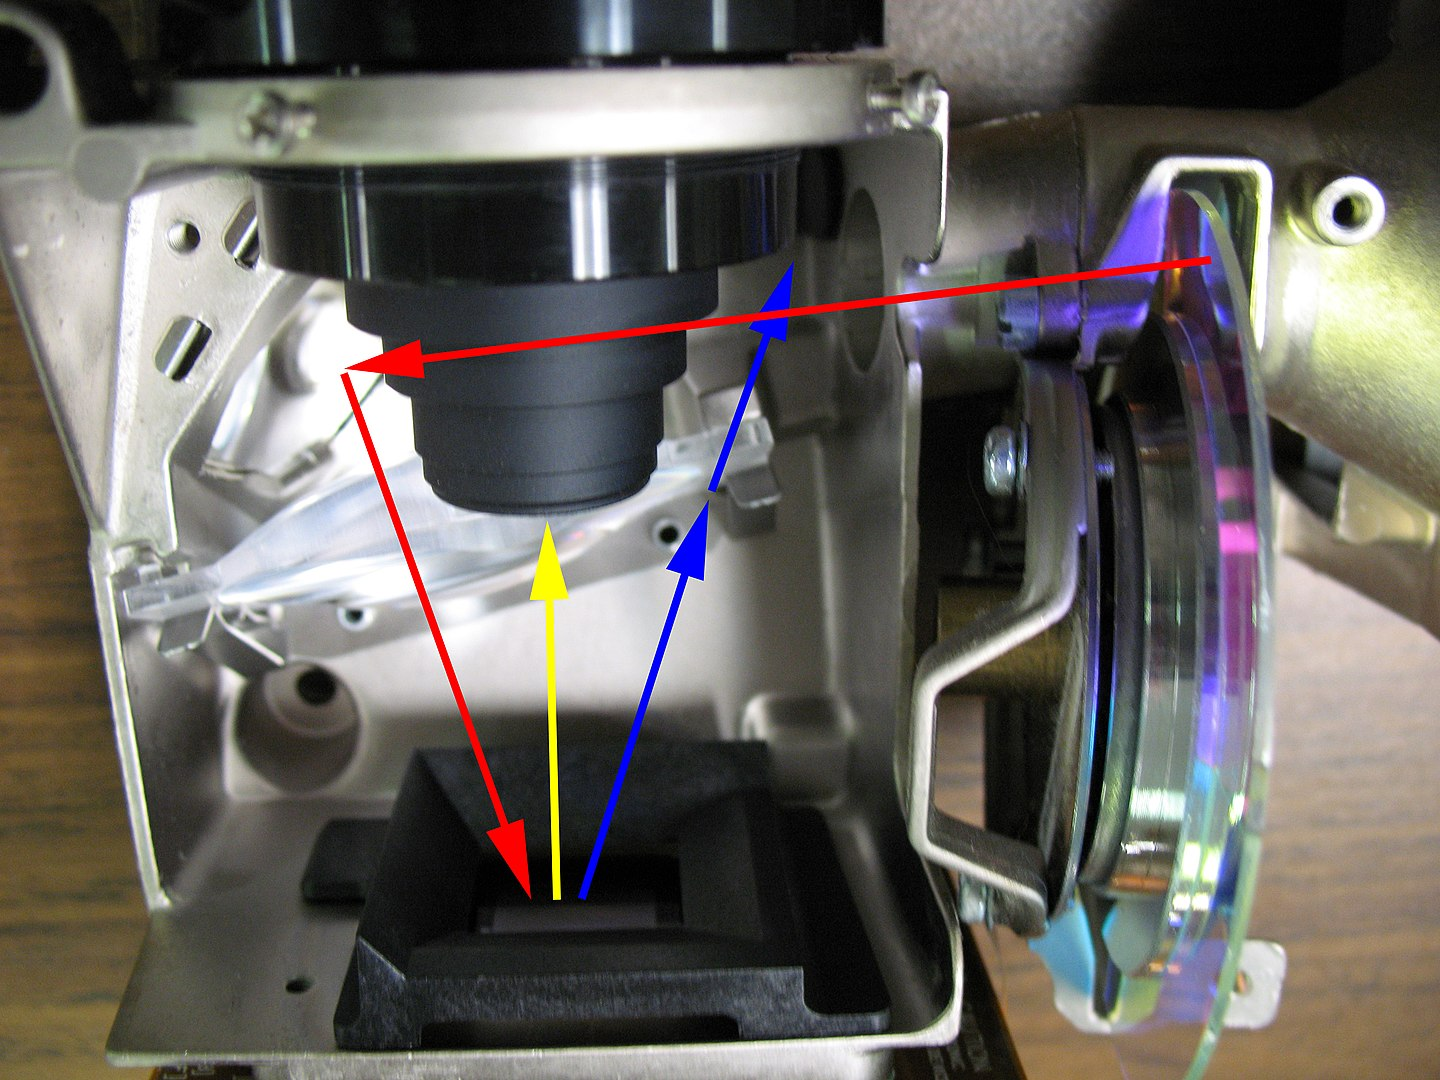
\includegraphics[width=\textwidth]{images/02-projector_dlp.jpg}
        \caption{Source: \citet{ImageProjectorDLP}}
        %\label{}
    \end{subfigure}
    \hfill
    \begin{subfigure}[b]{0.49\textwidth}
        \centering
        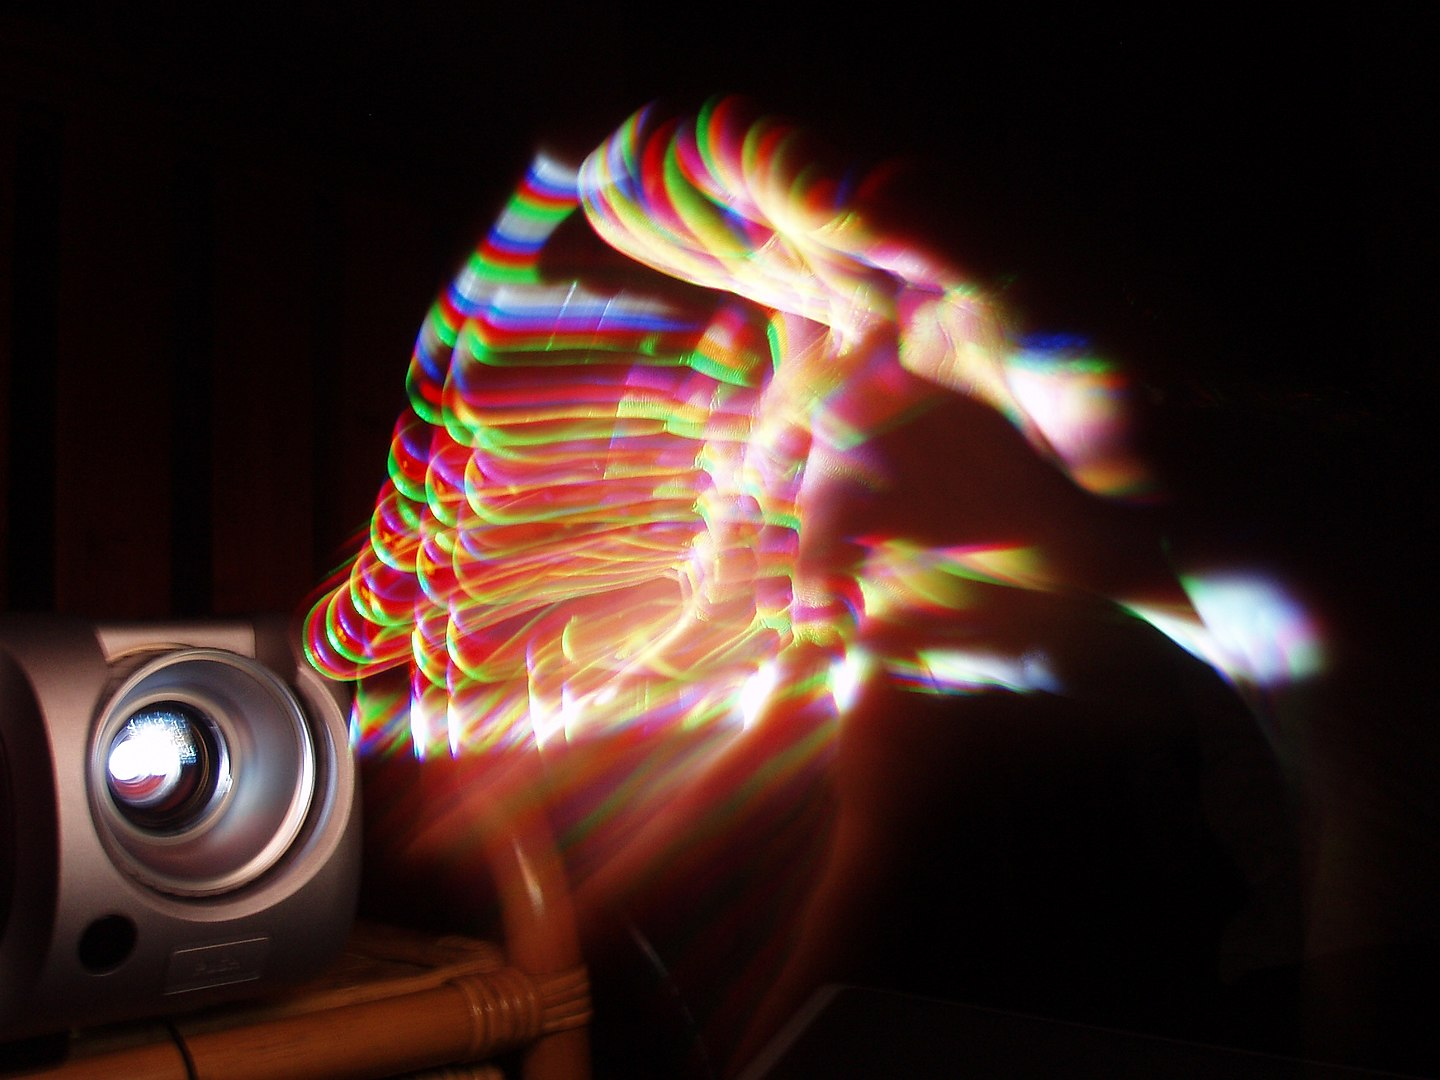
\includegraphics[width=\textwidth]{images/02-projector_rainbow.JPG}
        \caption{Source: \citet{ImageProjectorDLPRainbow}}
        %\label{}
    \end{subfigure}
    \caption{Image a) shows how a DLP projector works. First, bright white light passes through the color wheel. Then it is reflected off the the DMD (red arrows) into either the lens (yellow arrow), or the heat sink (blue arrows). Image b) shows how a DLP projector with a single DMD chip sends out single channel images in rapid succession. This can result in artifacts which can be fixed by using a separate DMD chip for each primary color}
    \label{fig:background_projector_dlp}
\end{figure}

\subsubsection{Gamut Limitations}
\label{section:background-projection_mapping-projectors-limitations}

Based on the way DLPs work, it is easy to see that the process of projecting an image is fairly inefficient since a bright white light is emitted at all times and based on the image being displayed a portion of it is sent into the heat sink and wasted. The main two limitations that result from this and that we are concerned with when projection mapping are limited maximum and minimum brightness.

Maximum brightness is simply limited by the brightness of the lamp. The brighter the lamp, the more energy it consumes and the less efficient it becomes when dark images are being projected.

Minimum brightness is related to the ability of the projector to absorb light which is not reflected directly towards the lens. The more light is absorbed inside the projector, the more the projector heats up. This is why DLP projectors with deep blacks need to be large enough to cool themselves down efficiently. If a DLP projector is not able to absorb all the light, some of it is let through towards the screen and results in dim gray instead of the intended black.

Different projector technologies have different limitations. For example, laser projectors are generally more efficient and brighter because they produce exactly the light color which is needed, as opposed to filtering out white light. But even laser projectors cannot be infinitely bright nor can they subtract light from externally illuminated scenes.

Moreover, even if a particular color lies within the gamut of our projector, the scene that we are projecting onto might prevent us from reproducing that color faithfully. The study of how light interacts with matter to influence what we see around us is called the \textit{light transport theory}. We provide a brief introduction to it in order to understand what our projections look like and which colors are and are not reproducible with a particular scene and projector. But because this theory is rather complex, we begin by building intuition on what to roughly expect when we install a projector and press Play.

{\color{red} TODO: DoF and the thin lens model? (also a limitation that's relevant for us) also pinhole!}

\subsection{Intuition on Projection Appearance}
\label{section:background-projection_mapping-projection_intuition}

The appearance of an object is given by the light it reflects. Light is the visible portion of electromagnetic radiation and consists of photons at various wavelengths. Wavelengths which human vision is sensitive to are approximately between 380 and 780 nm (\citet{PBRT3e}). Shorter wavelengths appear blue, middle ones are green and longer ones are red. Reflectance of an object is defined by the so-called \textit{spectral power distribution} (SPD) which describes what proportion of incoming light is reflected at each wavelength.

\begin{figure}[ht]
    \centering
    \begin{subfigure}[b]{0.49\textwidth}
        \centering
        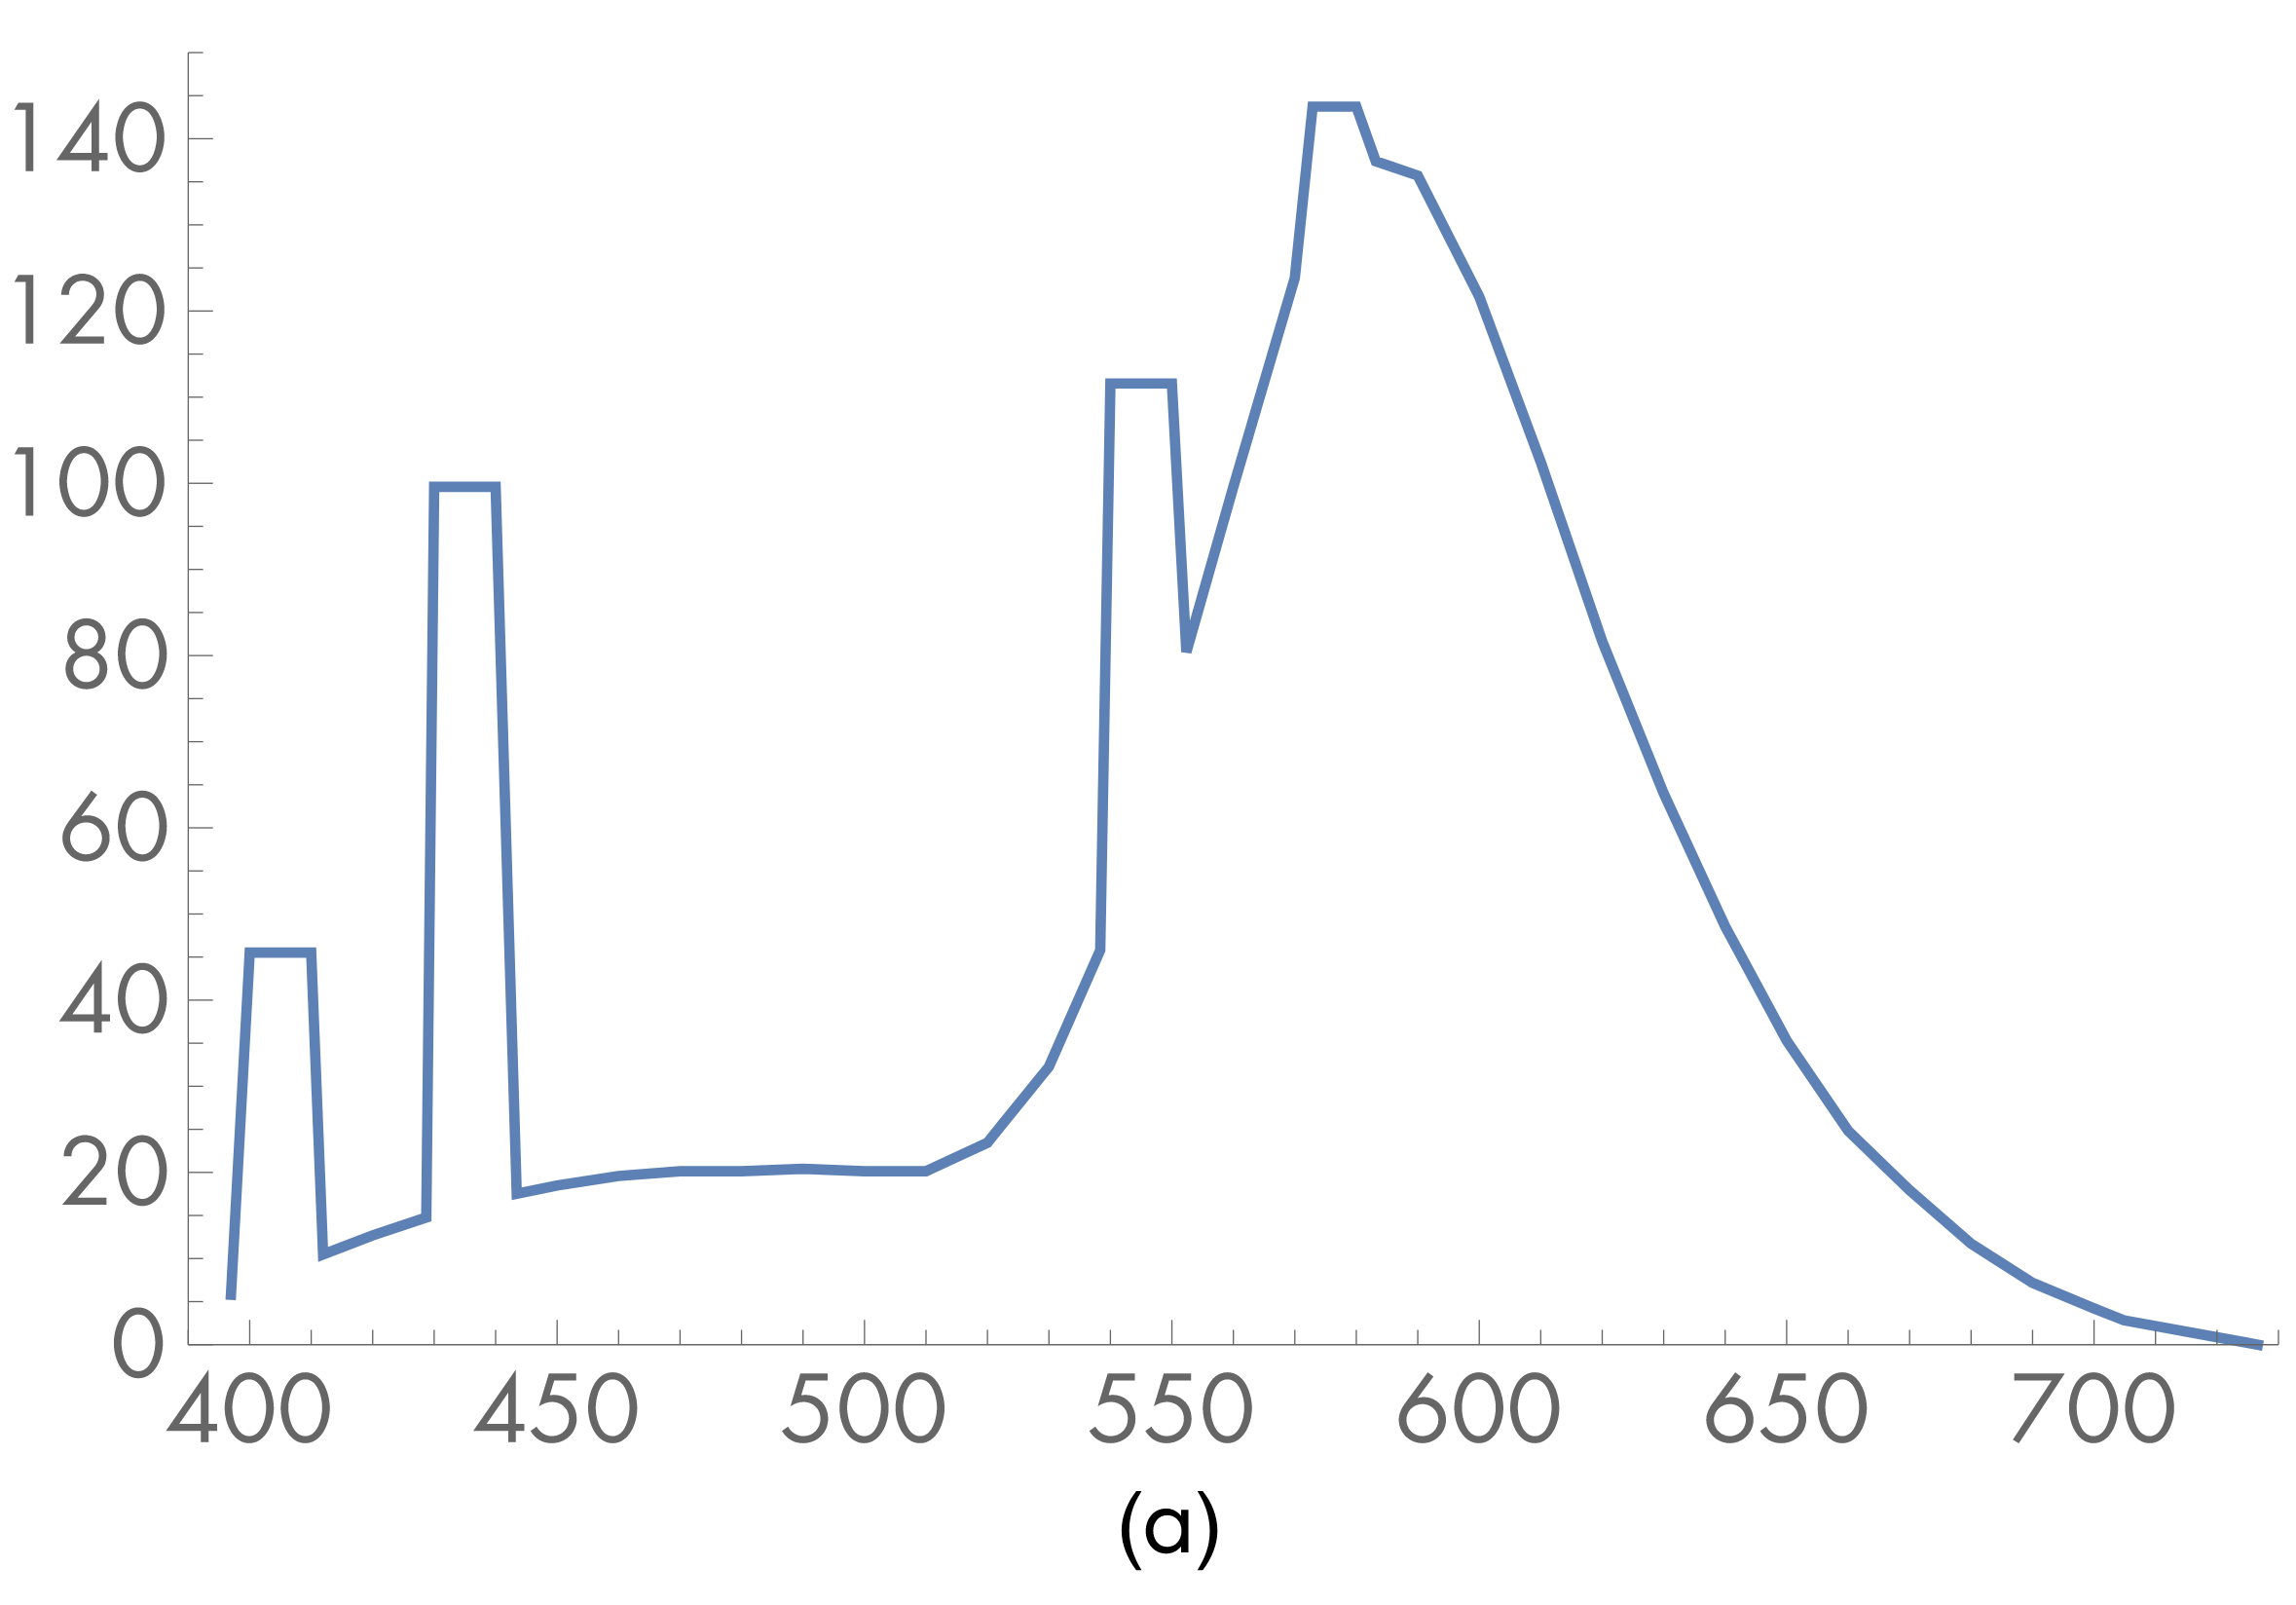
\includegraphics[width=\textwidth]{images/02-spd_fluorescent_light.png}
        \caption*{}
        %\label{}
    \end{subfigure}
    \hfill
    \begin{subfigure}[b]{0.49\textwidth}
        \centering
        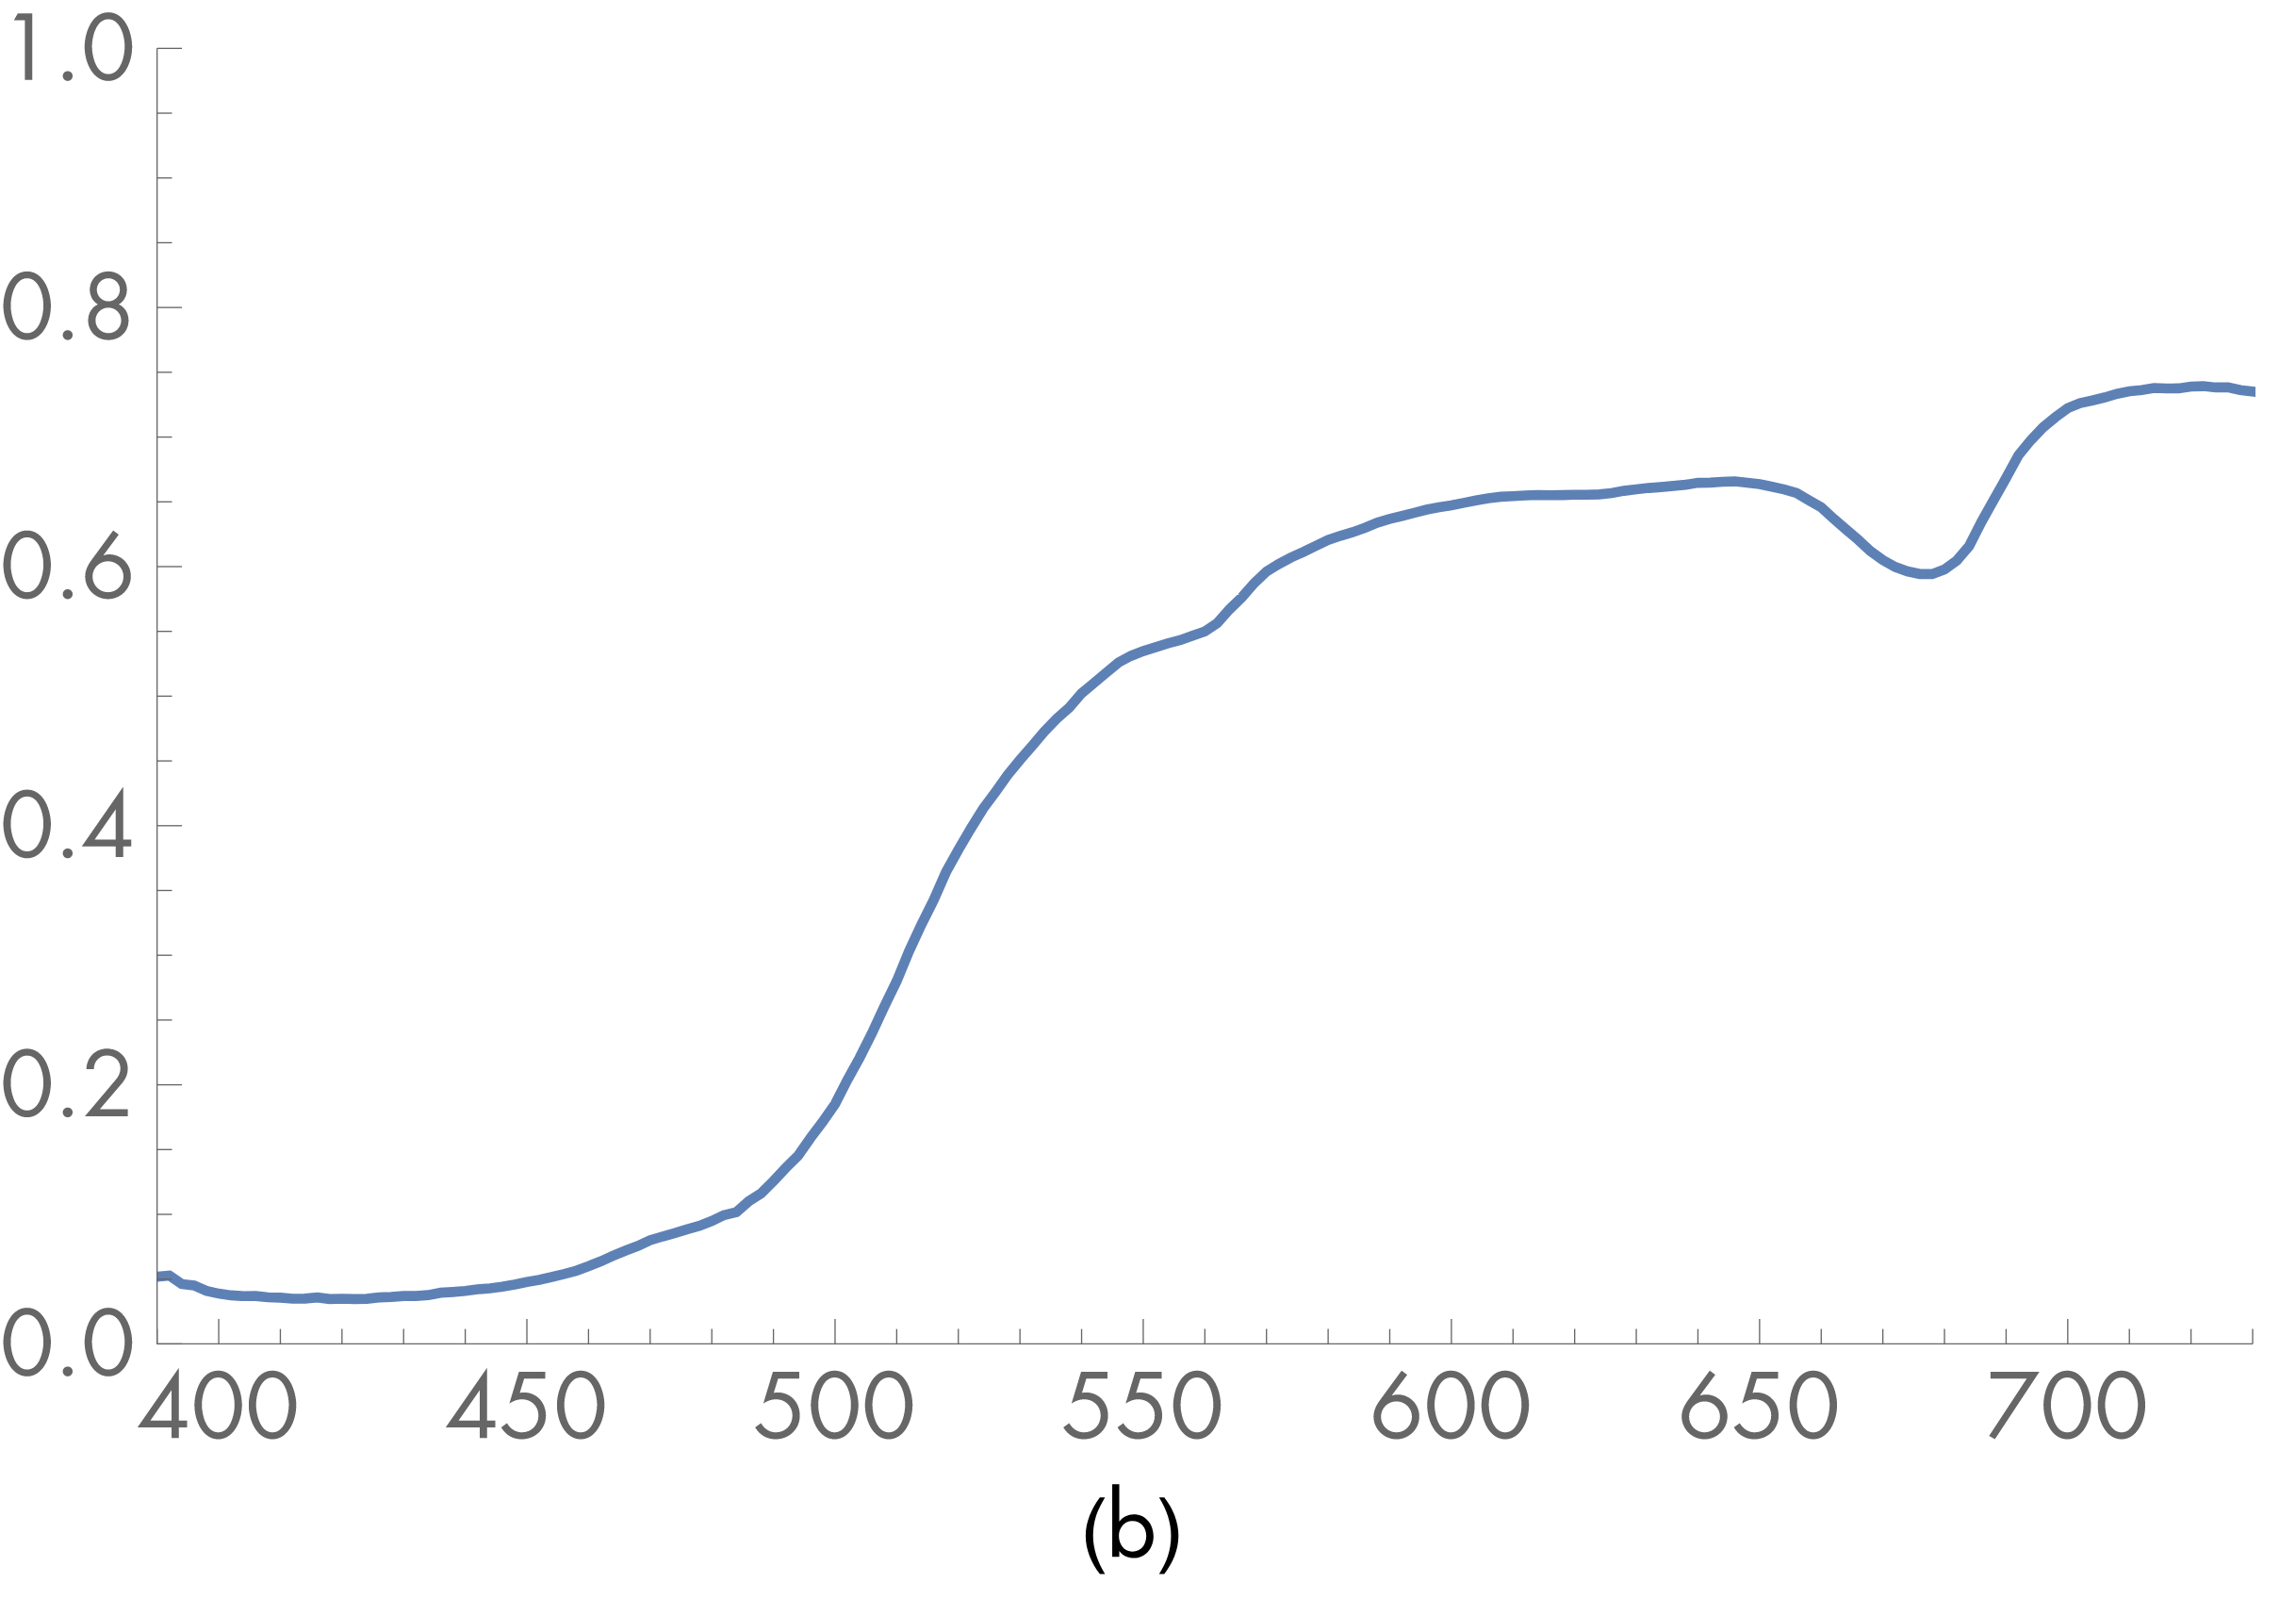
\includegraphics[width=\textwidth]{images/02-spd_lemon_peel.png}
        \caption*{}
        %\label{}
    \end{subfigure}
    \caption{Image a) shows the SPD of fluorescent light with power on the y-axis. Image b) shows the SPD of a lemon peel. Lemon peel is not an emitter hence the y-axis shows the proportion of wavelengths that are reflected off its surface. Source: \citet{PBRT3e}}
    \label{fig:background_spd}
\end{figure}

Projectors are above all light sources. As a matter of fact, each of the millions of tiny mirrors inside the DMD of a DLP projector can be thought of as a separate light source. Projector light has an SPD of its own, describing how much power it carries at each wavelength. When it interacts with a surface, something roughly corresponding to SPD multiplication takes place. If an object does not reflect any light at 450 nm, for example, all of it will be absorbed and will not reach our eyes. See fig. \ref{fig:background_spd_intuition} for examples of how projection interacts with various backgrounds.

\begin{figure}[ht]
    \centering    
    \begin{subfigure}{\textwidth}
        \centering
        \begin{subfigure}{0.24\textwidth}
            \centering
            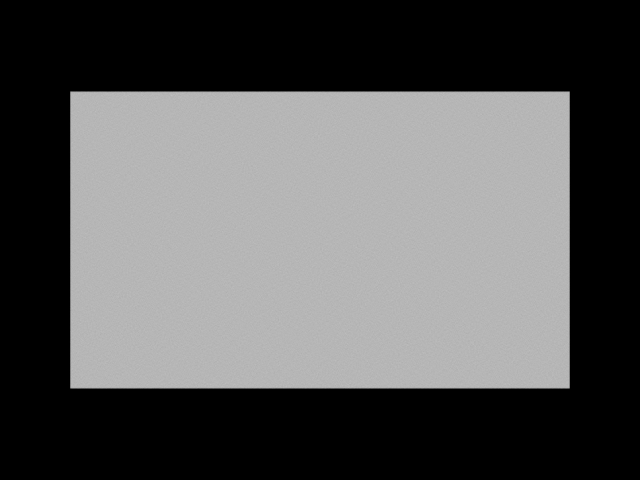
\includegraphics[width=\textwidth]{images/02-spd_intuition-white_white.png}
            \caption*{}
            \label{fig:background_spd_intuition-white_white}
        \end{subfigure}
        \hfill
        \begin{subfigure}{0.24\textwidth}
            \centering
            
\includegraphics[width=\textwidth]{images/02-spd_intuition-white_red.png}
            \caption*{}
            \label{fig:background_spd_intuition-white_red}
        \end{subfigure}
        \hfill
        \begin{subfigure}{0.24\textwidth}
            \centering
            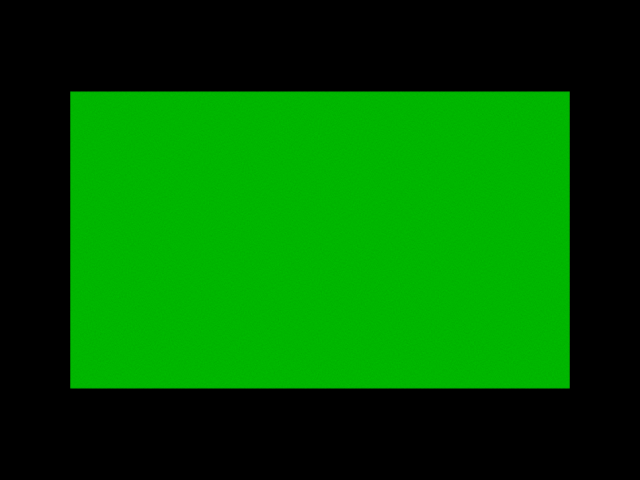
\includegraphics[width=\textwidth]{images/02-spd_intuition-white_green.png}
            \caption*{}
            \label{fig:background_spd_intuition-white_green}
        \end{subfigure}
        \hfill
        \begin{subfigure}{0.24\textwidth}
            \centering
            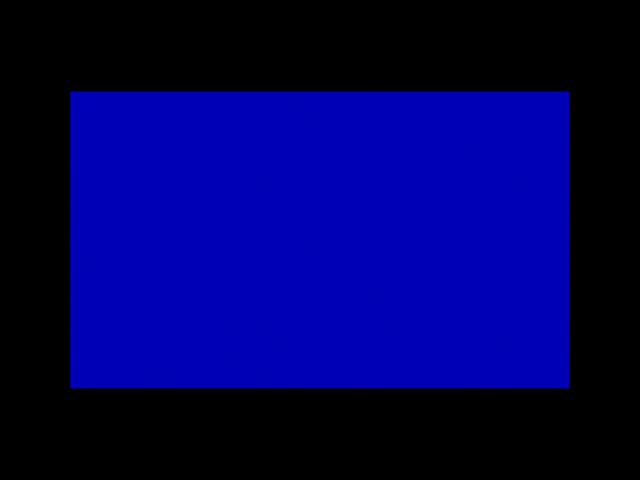
\includegraphics[width=\textwidth]{images/02-spd_intuition-white_blue.png}
            \caption*{}
            \label{fig:background_spd_intuition-white_blue}
        \end{subfigure}
        
        \begin{subfigure}{0.24\textwidth}
            \centering
            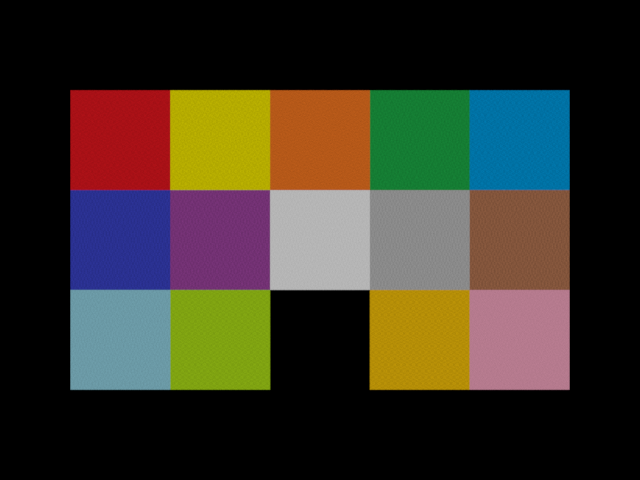
\includegraphics[width=\textwidth]{images/02-spd_intuition-palette_white.png}
            \caption*{}
            \label{fig:background_spd_intuition-palette_white}
        \end{subfigure}
        \hfill
        \begin{subfigure}{0.24\textwidth}
            \centering
            
\includegraphics[width=\textwidth]{images/02-spd_intuition-palette_red.png}
            \caption*{}
            \label{fig:background_spd_intuition-palette_red}
        \end{subfigure}
        \hfill
        \begin{subfigure}{0.24\textwidth}
            \centering
            
\includegraphics[width=\textwidth]{images/02-spd_intuition-palette_green.png}
            \caption*{}
            \label{fig:background_spd_intuition-palette_green}
        \end{subfigure}
        \hfill
        \begin{subfigure}{0.24\textwidth}
            \centering
            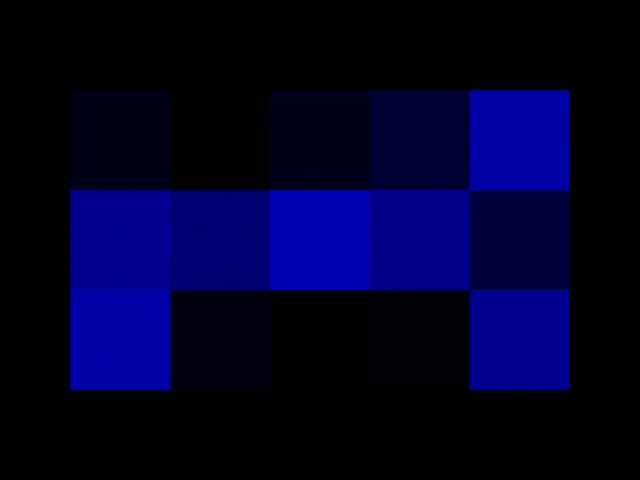
\includegraphics[width=\textwidth]{images/02-spd_intuition-palette_blue.png}
            \caption*{}
            \label{fig:background_spd_intuition-palette_blue}
        \end{subfigure}
    \end{subfigure}
    \caption{In the upper row, white light is projected onto a pure white, red, green and blue wall respectively. In the lower row, a color palette is projected onto the same backgrounds. Note that summing the last three images in each row gives the first one because each background has maximum reflectivity in one color channel and zero reflectivity in others. If a single-chip DLP projector were to project the first image, it would in fact send out the last three in rapid succession.}
    \label{fig:background_spd_intuition}
\end{figure}

We will now study this process more carefully using light transport theory.

\subsection{Light Transport Theory}
\label{section:background-projection_mapping-light_transport}

Light transport theory is the study of how light interacts with matter -- how it travels through space, scatters in fog, reflects from surfaces, refracts in camera lenses and absorbs in black T-shirts in summer. One of the most common uses of light transport is in architectural visualizations (see fig. \ref{fig:background_light_transport_examples-rendering}) and video game and movie rendering. There, we are interested in the SPD that arrives at each pixel of a virtual camera given geometry, materials and light sources.

\begin{figure}[ht]
    \centering
    \begin{subfigure}[b]{0.56\textwidth}
        \centering
        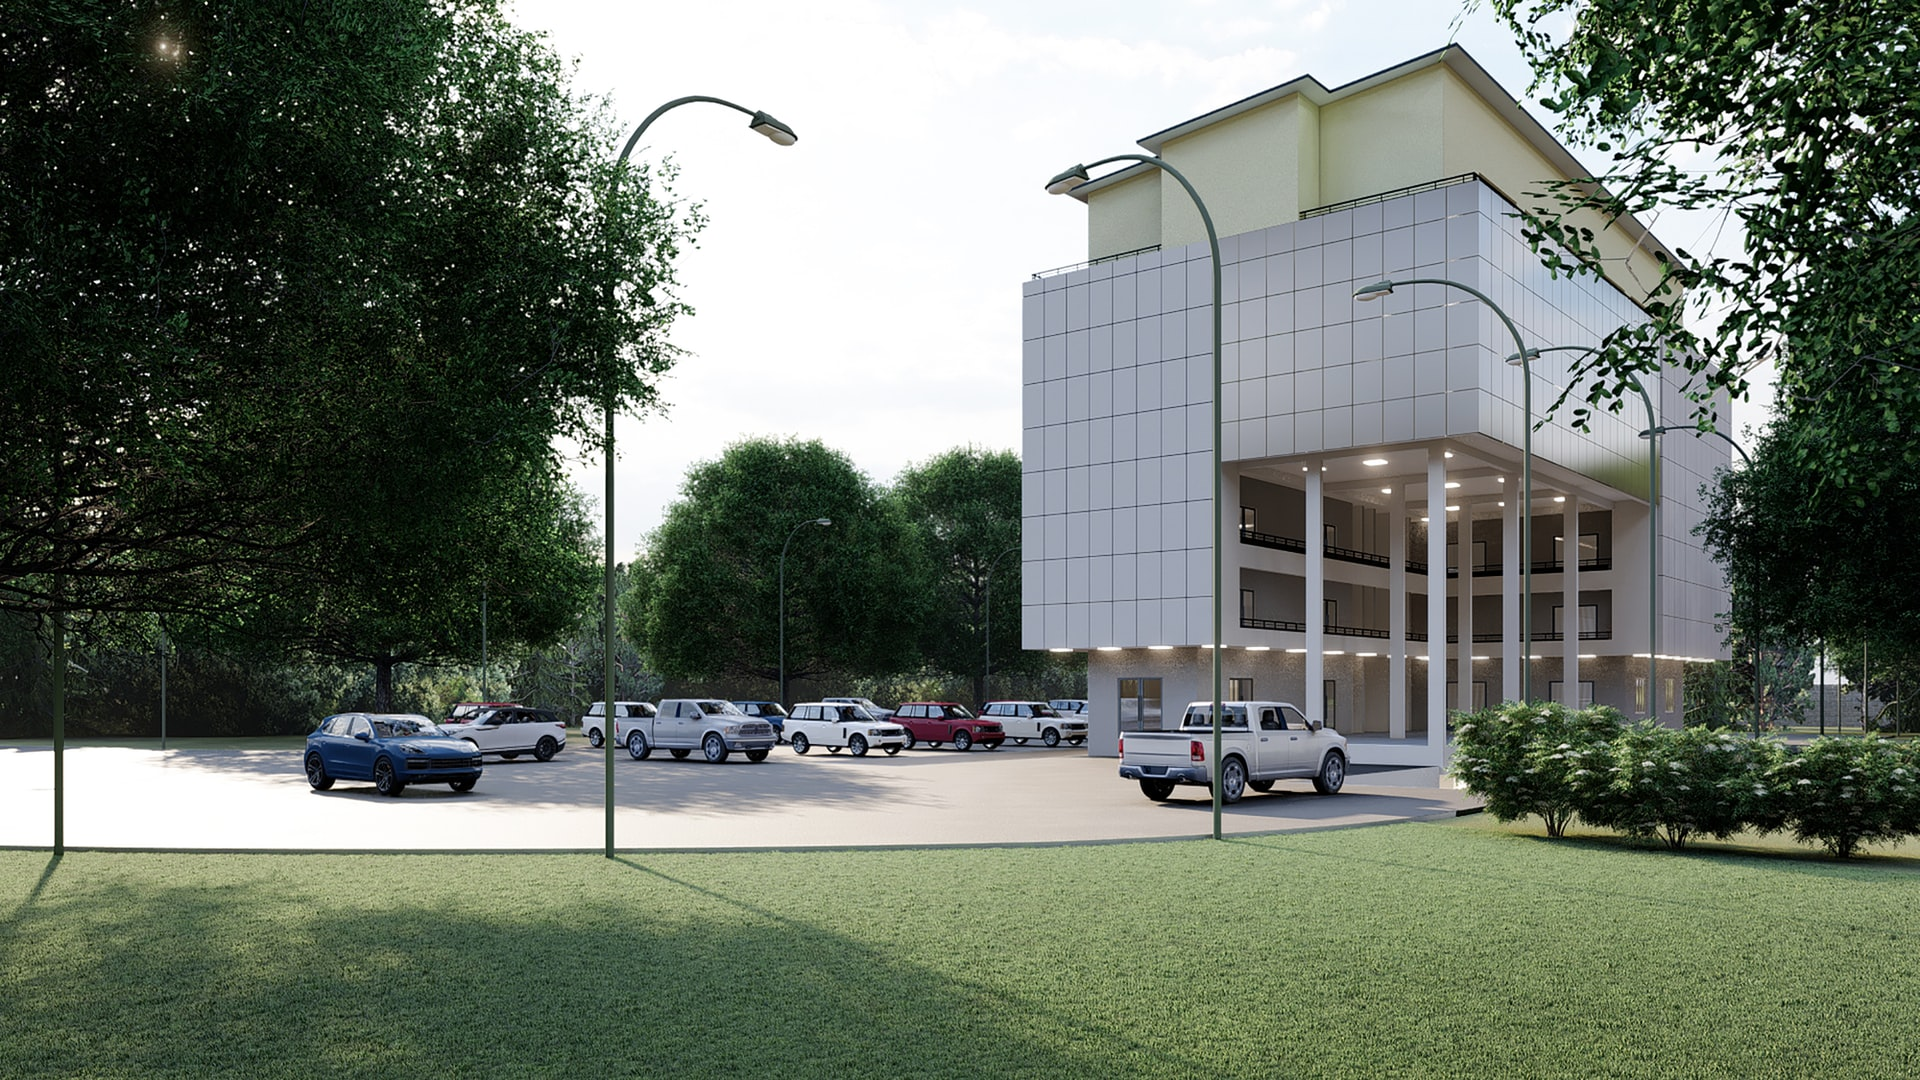
\includegraphics[width=\textwidth]{images/02-rendering.jpg}
        \caption{Source: \citet{ImageRendering}}
        \label{fig:background_light_transport_examples-rendering}
    \end{subfigure}
    \hfill
    \begin{subfigure}[b]{0.42\textwidth}
        \centering
        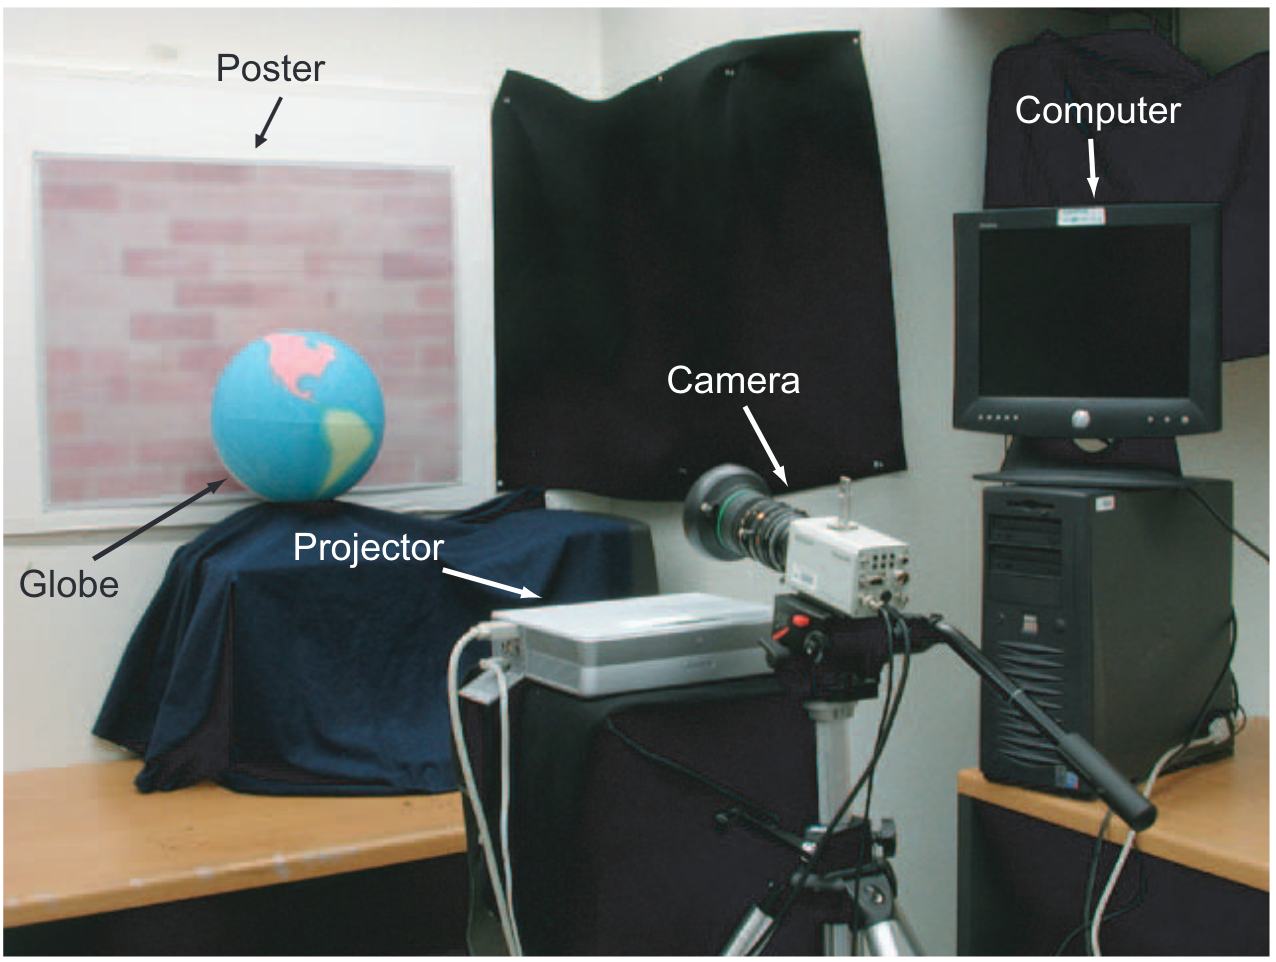
\includegraphics[width=\textwidth]{images/01-procam.png}
        \caption{Source: \citet{Grossberg2004}}
        \label{fig:background_light_transport_examples-procam}
    \end{subfigure}
    \caption{Image a) is an architectural visualization which uses light transport theory to solve the following problem: Given scene geometry, materials and light sources and camera position, what will the camera see? Image b) is a projector-camera system calibration from section \ref{section:intro-problem_setting} and asks: Given what the camera sees when various patterns are projected onto the scene, what can we say about the geometry and materials of the scene?}
    \label{fig:background_light_transport_examples}
\end{figure}

In this section, we provide a brief overview of light transport theory and explain how it can be used in projection mapping. For a more comprehensive coverage, we refer the reader to Physically Based Rendering: From Theory to Implementation by \citet{PBRT3e}.

\subsubsection{Radiance}
\label{section:background-projection_mapping-light_transport-radiance}

As mentioned in \ref{section:background-projection_mapping-projection_intuition}, all we see is light. Measuring light is therefore the crux of understanding how things look. The fundamental quantity we are interested in when measuring light is \textit{radiance}. It is defined as the amount of photons \(Q\) per unit projected area \(A^\perp \) per unit solid angle \(\omega\) per unit of time \(t\) (see fig. \ref{fig:background_radiance}):

\begin{equation}
    \label{eq:radiance}
    L = \frac{dQ}{dA^\perp d\omega dt}
\end{equation}

\begin{figure}[ht]
    \centering
    \def\svgwidth{0.8\textwidth}
    \input{images/figures/02-radiance.pdf_tex}
    \caption{Illustration of radiance which is defined as the amount of photons \(Q\) per unit projected area \(A^\perp \) per unit solid angle \(\omega\) per unit of time \(t\)}
    \label{fig:background_radiance}
\end{figure}

As suggested in fig. \ref{fig:background_spd}, to see the full picture, we need to consider radiance at each visible wavelength. A common approach to simplifying this is decompose the space of all visible SPDs into three basis functions which roughly correspond to red, green and blue colors. In that case, we would be interested in radiance in each of these channels. To simplify our explanations even further, we only talk about radiance \(L\). It is, however, important to realize that there is a layer of complexity hidden behing that notation.

Another issue with radiance is that it is a purely physical quantity while how we perceive something is to do with psychology. Luckily, for each radiometric measurement, such as radiance, there is a corresponding \(photometric\) measurement which expresses how a stimulus is perceived by the human visual system. The photometric counterpart to radiance is \(luminance\) and can be obtained from radiance by integrating against an empirically constructed spectral response curve which describes how the human eye reacts to various wavelengths. Because luminance can be easily computed from radiance, we only discuss radiance in this thesis.

We will now present the relationship between objects, light sources and the radiance incoming onto our camera sensor or eye retina. This relationship sits at the heart of light transport theory and is called the \textit{rendering equation}.

\subsubsection{Rendering Equation}
\label{section:background-projection_mapping-light_transport-rendering_equation}

The rendering equation describes the amount of outgoing radiance from point \(x\) in a scene towards a direction \(\mathbf{v}\):

\begin{equation}
    \label{eq:rendering_equation}
    L(x \rightarrow \mathbf{v}) = \int_{\Omega(x)} L(x \leftarrow \mathbf{u}) f_r(x, \mathbf{u} \rightarrow \mathbf{v}) \cos \theta d\mathbf{u} + E(x \rightarrow \mathbf{v})
\end{equation}

{\color{red} TODO: figure of rendering equation}

where \(L(x \leftarrow \mathbf{u})\) is the radiance arriving at \(x\) from direction \(\mathbf{u}\), \(\Omega(x)\) is the hemisphere oriented to the direction of the surface normal at \(x\), \(f_r\) is the spatially-varying bidirectional reflectance distribution function (SVBRDF) which determines surface reflectance for each point \(x\), incoming direction \(\mathbf{u}\) and outgoing direction \(\mathbf{v}\), and \(\theta\) is the angle between \(u\) and the surface normal at \(x\). Finally, \(E(x \rightarrow \mathbf{v})\) is the radiance emitted from \(x\) towards \(\mathbf{v}\) in case \(x\) lies on a light source.

The main idea of the equation is that radiance leaving towards \(\mathbf{v}\) from \(x\) is the sum of reflected and emitted radiance. It assumes empty space between objects, therefore no light scattering occurs between them. This means that radiance is constant along straight lines and the equation is recursive -- \(L(x \leftarrow \mathbf{u}) = L(y \rightarrow -\mathbf{u})\) where \(y\) is the point seen from \(x\) in the direction of \(\mathbf{u}\). Generalizations of the rendering equation to scenes with participating media where this is not the case are discussed in a SIGGRAPH course by \citet{Novak2018}.

Apart from assuming that our objects are in vacuum, the equation also assumes that light is reflected from the same point it arrived at. This is generally not the case as can be seen for example with human skin where light bounces under the surface before it is reflected. This phenomenon is known as \textit{subsurface scattering} and a generalization of the rendering equation to account for it has been presented for example by \citet{Jensen2001}. For our purposes, however, it is sufficient to be familiar with the basic form of the rendering equation.

To determine the amount of radiance that hits a virtual camera sensor in scenes such as fig. \ref{fig:background_light_transport_examples-rendering}, we need to solve the rendering equation for points that lie on the sensor and directions towards points in the scene that are visible from the sensor. This is typically done by Monte Carlo integration which estimates the integral by random sampling. Each sample is a light path from a light source towards the camera with zero or more bounces on the surfaces of the scene. A strategy to choose such samples is crucial to the performance of a rendering algorithm. A brilliant overview of sampling strategies, for example bidirectional path tracing (BDPT) can be found in \citet{Veach1997}.

\subsubsection{Towards Projection Mapping}
\label{section:background-projection_mapping-light_transport-towards_projection_mapping}

In a sense, projection mapping is a more difficult problem than rendering. Whereas in rendering, the scene geometry, materials and light sources are known and the radiance at the camera sensor is unknown, in projection mapping we only know the radiance at the camera sensor and everything else, including the projection image (our light source), is unknown.

{\color{red} TODO: figure that compares rendering to projection mapping}

Projection mapping algorithms therefore do not typically solve the full (inverse) light transport of the whole scene, but instead they build on top of assumptions and provide estimates. Common assumptions are for example

\begin{itemize}
    \item A known relationship between the projector and camera orientation
    \item Absence of glossy surfaces whose appearance depends on view point
    \item A 1:1 correspondence between projector and camera pixels, meaning that each pixel of the camera image is influenced by only one projector pixel. Note that this does not hold for example in scenes with convex geometry where light from multiple projector pixels is concentrated into a single camera pixel
\end{itemize}

We will now review some common approaches to projection mapping found in state-of-the-art methods. Our goal is to use this information to construct a reference method that we can implement in our projector-camera system simulator and use in experiments to compare our proposed projection mapping method against.

\subsection{Projector-Camera Systems}
\label{section:background-projection_mapping-procams}

The key idea in projection mapping is to use a camera to observe the projection and provide information on how to adapt it to achieve desired appearance. This system as a whole is called the \textit{projector-camera system}, commonly shortened as \textit{procam}.

As mentioned in eq. \ref{eq:projection_mapping-per_pixel}, this adaptation is done by modifying the projector image until the camera image matches the desired appearance pixel by pixel. However, the relationship between projector and camera pixels is very complex, as suggested in section \ref{section:background-projection_mapping-light_transport} on light transport theory. The model of this relationship is the main differentiating factor of various projection mapping methods.

On a high level, projection mapping methods can be split into two groups:

\begin{itemize}
    \item Those that assume a 1:1 correspondence between projector and camera pixels
    \item Those that do not and instead attempt to solve general light transport in the whole scene
\end{itemize}

The first group usually has two smaller tasks to perform. First, they need to establish those correspondencies geometrically in a step called \textit{geometric calibration}. Then, they need to model how the intensity of a projector pixel affects the intensity of the corresponding camera pixel in a step called \textit{radiometric calibration}. Despite the original assumption of 1:1 pixel correspondence, these methods are reasonably general and work quite well. They are also the most common. We will therefore review a few of them and focus on how projector hardware (along with scene complexity) limits their performance.

The second group typically uses \textit{inverse light transport} to model the relationship between projector and camera as generally as possible. These methods are mostly limited by the computational complexity of such a task. Some, for example \citet{Siegl2017}, achieve real time performance at the cost of using an additional depth camera to gain more information about the scene and projecting only on matte objects of constant color. We will focus on an older method by \citet{Wetzstein2007} that works with arbitrarily complex scenes and will thus be useful for us when constructing our reference method.

For a complete overview of the state of the art in projection mapping, see \citet{Grundhofer2018}.

\subsubsection{Geometric Calibration}
\label{section:background-projection_mapping-procams-geometric_calibration}

The goal of geometric calibration is to find a point \(M_c = [u_c, v_c]^T\) in the camera image for each point \(M_p = [u_p, v_p]^T\) in the projector image such that the value of the latter determines the value of the former. These correspondencies are usually established via a third point, \(P = [x, y, z]\) which is located in the scene.

The relationship between \(M_c\) and \(P\) is determined by the \textit{intrinsic} and \textit{extrinsic} matrices:

\begin{equation}
    \label{eq:camera_equation}
    \begin{bmatrix}
        u_c \\
        v_c \\
        1
    \end{bmatrix} =
    \begin{bmatrix}
        f_x & s & u \\
        0 & f_y & v \\
        0 & 0 & 1 
    \end{bmatrix} \cdot
    \begin{bmatrix}
        \mathbf{R} & \mathbf{t}
    \end{bmatrix} \cdot
    \begin{bmatrix}
        x \\
        y \\
        z
    \end{bmatrix}
\end{equation}

where the intrinsic matrix is formed by camera focal lengths \(f_x\) and \(f_y\) (focal length is expressed in pixels and if pixels are square, then \(f_x = f_y = f\)), skewness \(s\) of image axes, and principal point coordinates \([u, v]^T\) (the intersection of optical axis and image plane which is generally not in the center of the image). The extrinsic matrix is then formed by rotation \(\mathbf{R}\) and translation \(\mathbf{t}\) which convert between world coordinates and camera coordinates. See fig. \ref{fig:background_camera_calibration} for an illustration.

\begin{figure}[ht]
    \centering
    \def\svgwidth{0.8\textwidth}
    \input{images/figures/02-camera_calibration.pdf_tex}
    \caption{Illustration of geometric calibration of projector and camera. Points \(M_c\) and \(M_p\) on camera and projector image plane, respectively, are related via a point \(P\) in the scene. \(f\) is the focal length which is the distance between pinhole and principle point and \(u\) and \(v\) are principle point coordinates with respect to image plane origin}
    \label{fig:background_camera_calibration}
\end{figure}

The most commonly used method for finding the parameters of eq. \ref{eq:camera_equation} was introduced by \citet{Zhang1999}. They are estimated by taking at least two photos of a planar pattern at various orientations.

We will now outline two recent methods to perform geometric calibration. The first one requires user assistance, while the second one is fully automatic.

\textbf{One camera, one projector and a calibration board.} The first method, introduced by \citet{Yang2016}, uses a calibration board containing a random dot pattern. First, the camera is calibrated using the approach of \citet{Zhang1999}. Then the projector is calibrated by projecting another dot pattern onto the board and treating the projector as an inverse camera. The whole process needs around 10 views of the calibration board according to experiments in the paper.

\textbf{Two cameras, one projector.} An entirely automatic self-calibration method was presented by \citet{Willi2017}. Their method first establishes pixel correspondencies between the two cameras and then continues to estimate the intrinsic and extrinsic matrix, as well as the 3D point cloud of the scene. Finally, the projector is calibrated using this information. It is worth noting that this method works also for any larger number of projectors and cameras in which case camera pairs are sorted by the quality of their pixel correspondencies. Calibration is first done for the best pair and other devices are incorporated iteratively, improving the overall estimate.

\subsubsection{Radiometric Calibration}
\label{section:background-projection_mapping-procams-radiometric_calibration}

Once correspondencies between projector and camera pixels have been established, radiometric calibration can be performed. In general, the goal is to find a color-mapping function \(f\) such that

\begin{equation}
    \label{eq:radiometric_calibration}
    \begin{bmatrix}
        C_R \\
        C_G \\
        C_B
    \end{bmatrix} = f(
        \begin{bmatrix}
            P_R \\
            P_G \\
            P_B
        \end{bmatrix}
    )
\end{equation}

where \(C\) is the color of a camera pixel and \(P\) is the color of the corresponding projector pixel. We describe one method that assumes \(f\) to be linear and one method that allows for arbitrary \(f\).

\textbf{Linear color-mapping function.} One of the first projection mapping methods was presented by \citet{Grossberg2004}. There, the relationship between \(c_c\) and \(c_p\) is specified as follows:

\begin{equation}
    \label{eq:linear_color_mapping}
    \begin{bmatrix}
        C_R \\
        C_G \\
        C_B
    \end{bmatrix} = p_c(
        \begin{bmatrix}
            V_{RR} & V_{RG} & V_{RB} \\
            V_{GR} & V_{GG} & V_{GB} \\
            V_{BR} & V_{BG} & V_{BB}
        \end{bmatrix} \cdot p_p(
            \begin{bmatrix}
                P_R \\
                P_G \\
                P_B
            \end{bmatrix}
        ) +
        \begin{bmatrix}
            F_R \\
            F_G \\
            F_B
        \end{bmatrix}
    )
\end{equation}

where \(p_p\) is a non-linear projector response function which turns input pixel values into projector brightness, \(p_c\) is a non-linear camera response that converts radiance arriving at the camera sensor to output pixel value, \(F = [F_R, F_G, F_B]^T\) is the environment light term which is independent of the projector, and finally \(V\) is a \(3 \times 3\) color mixing matrix which captures the relationship between projector and camera channels and their interactions with spectral reflectance.

Both \(p_p\) and \(p_c\) are independent of the scene and can be estimated separately. \(V\) and \(F\) are per-pixel and scene-dependent and can be estimated by projecting and capturing 6 calibration images.

The disadvantage of this method is that the linear color mixing matrix is not an accurate model for example when using DLP projectors described in section \ref{section:background-projection_mapping-projectors-DLP}. DLP projectors sometimes form an image by composing red, green, blue and white channels together. The extra white channel may result in non-linear behavior. Another disadvantage is related to projector brightness limitations. If the color gamut of the projector struggles to reproduce the color required by the compensation model, it results in clipping artifacts and lowered contrast. See fig. \ref{fig:background_clipping} for an illustration.

\begin{figure}[ht]
    \centering
    \def\svgwidth{0.6\textwidth}
    \input{images/figures/02-clipping.pdf_tex}
    \caption{Illustration of reduced contrast due to brightness limitations. Projector gamut is delimited by a triangle. If a compensation model requires a color which is outside the triangle, the closes color on the edge of the triangle is projected instead. Colors inside the triangle are projected as required which results in reduced contrast between the two groups}
    \label{fig:background_clipping}
\end{figure}

\textbf{Non-linear color-mapping function with a global optimization step.} To solve these problems, \citet{Grundhofer2015} presented an improved method which allows for an arbitrary color-mixing function. This function is estimated by obtaining up to \(6^3\) samples and then applying thin-plate spline interpolation on them. This sampling process takes several minutes but once it is completed, compensation can be performed in real time.

Moreover, the paper acknowledges that the contrast issues stem from the way the camera image is matched with the desired appearance pixel by pixel (see eq. \ref{eq:projection_mapping-per_pixel}). To fix this, it uses a global optimization step which compensates the image based on its higher level content. In this step, a patch size is chosen (typically \(2^n\) pixels) and a color-correcting coefficient is introduced for each patch. The coefficients are set so as to minimize clipping errors caused by limited color gamut of the projector and overall increase image contrast.

\begin{figure}[ht]
    \centering
    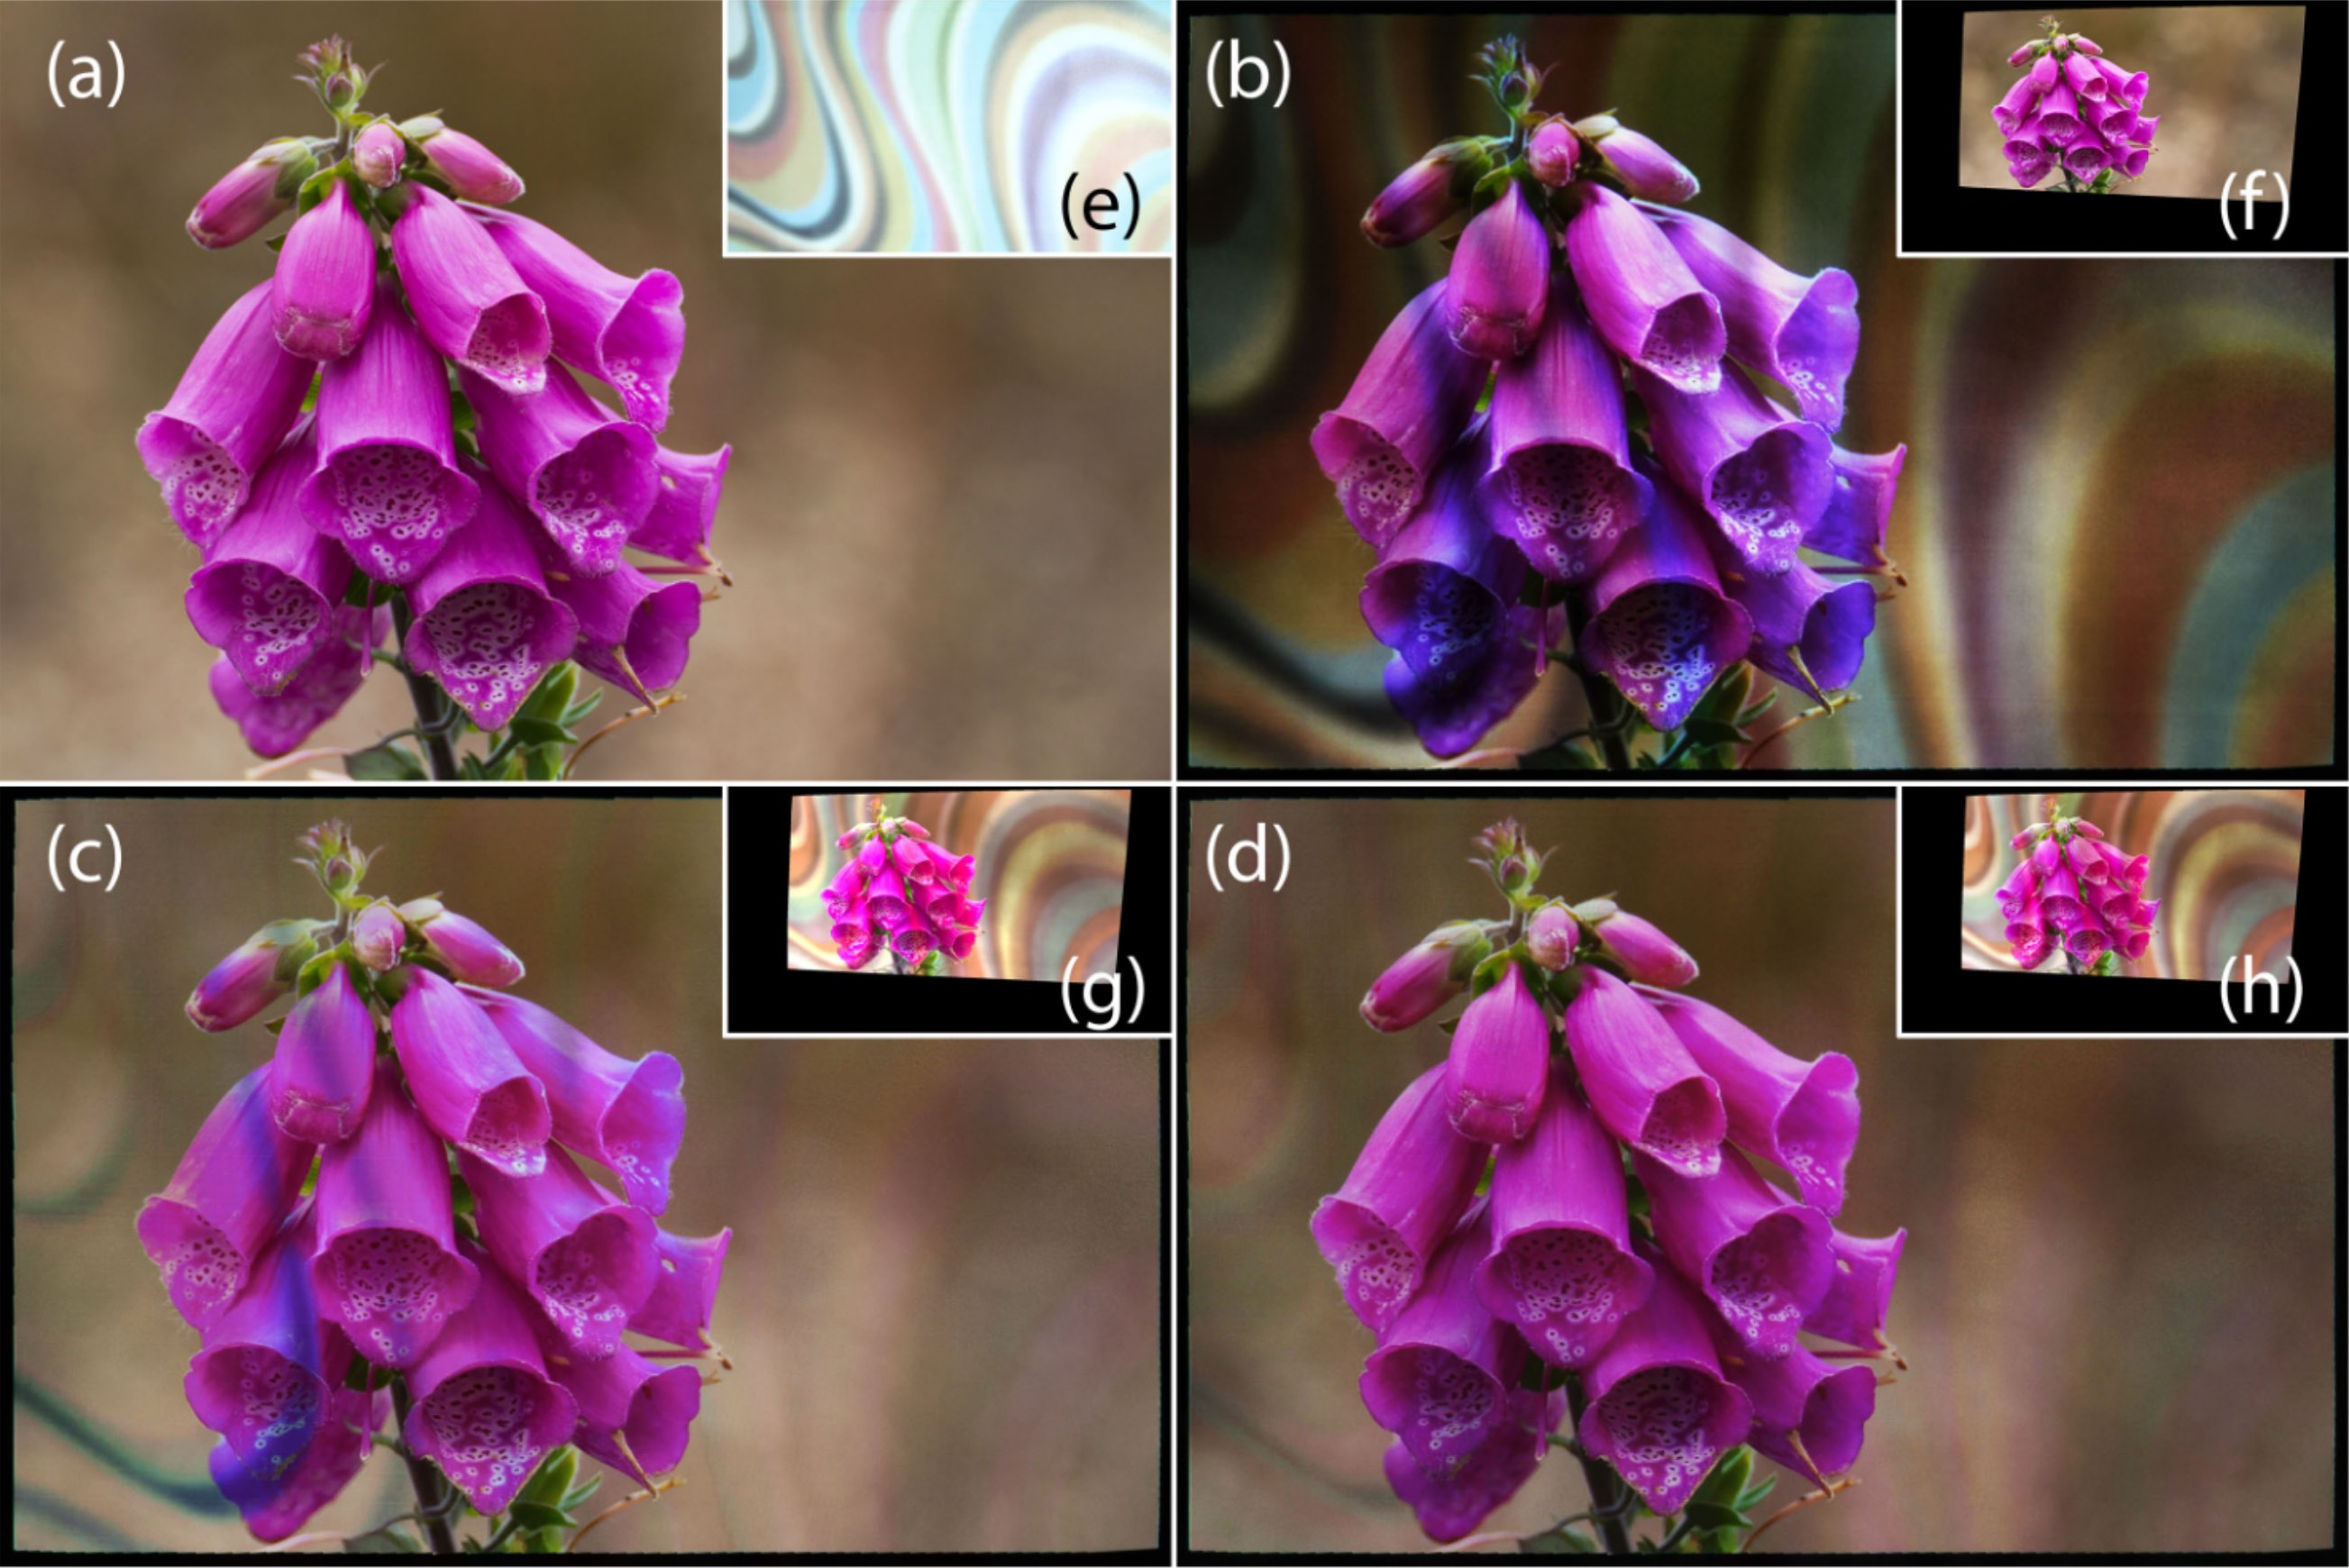
\includegraphics[width=0.6\textwidth]{images/02-grundhofer_result_compressed.jpg}
    \caption{Results of a projection mapping method by \citet{Grundhofer2015}. (a) original input image. (e) non-uniformly colored projection surface (illuminated  uniformly white). (b) captured projection of (a) on (e). (c) captured  projected  compensation  image shows local clipping errors. (d) reduced clipping errors after applying a global optimization step. (f-h) geometrically warped projection images generating camera images (b-d). Source: \citet{Grundhofer2015}}
    \label{fig:background_grundhofer_result}
\end{figure}

As a result, this method achieves very good results in scenes which have minimal inter-reflection that cannot be modeled when 1:1 correspondence between projector and camera pixels is assumed (see fig. \ref{fig:background_grundhofer_result}). The idea of the global optimization step is important because goes in the same direction as our method -- compensating the projection image not pixel by pixel, but based on higher-level content instead.

\subsubsection{Inverse Light Transport}
\label{section:background-projection_mapping-procams-inverse_lt}

Another approach to projection mapping that does not rely on the assumption of 1:1 correspondence between projector and camera pixels is so-called inverse light transport. The basic idea behind this approach is that radiance incoming onto camera sensor is a linear function of light sources in the scene. This can be derived directly from the rendering equation (see eq. \ref{eq:rendering_equation}) and practical examples can be seen in fig. \ref{fig:background_linear_lt}.

\begin{figure}[ht]
    \centering
    \begin{subfigure}[b]{0.24\textwidth}
        \centering
        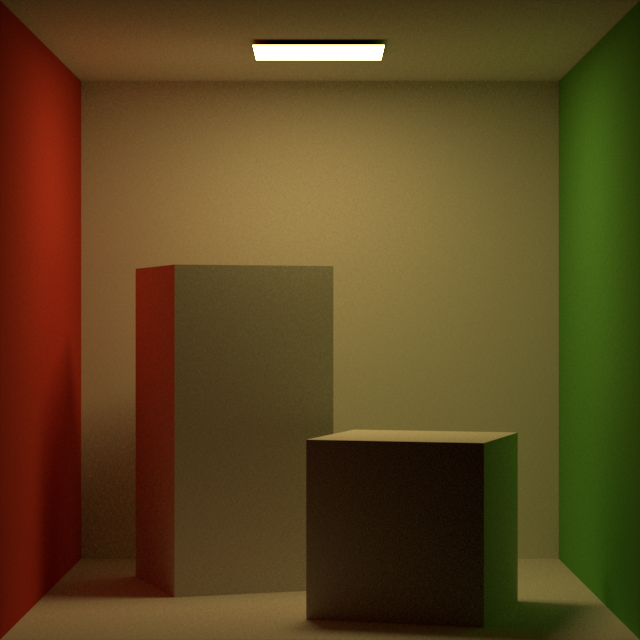
\includegraphics[width=\textwidth]{images/02-linear_lt_light01.jpg}
        \caption*{\(a = 1.0\), \(b = 0.0\)}
        %\label{}
    \end{subfigure}
    \hfill
    \begin{subfigure}[b]{0.24\textwidth}
        \centering
        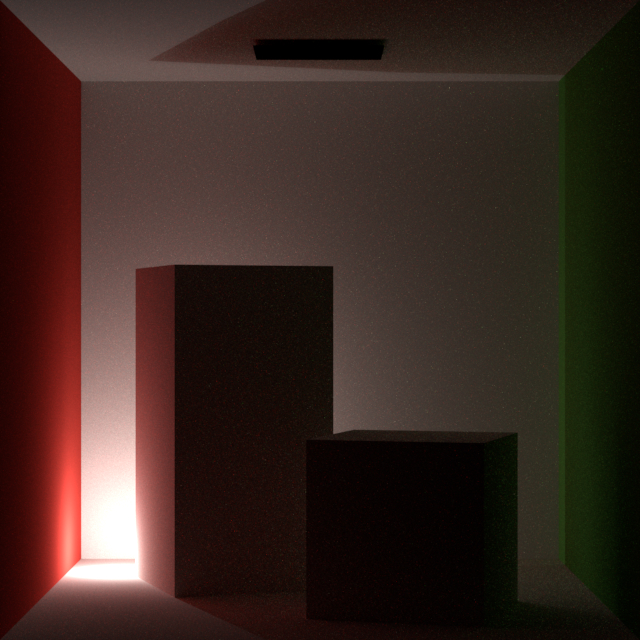
\includegraphics[width=\textwidth]{images/02-linear_lt_light02.jpg}
        \caption*{\(a = 0.0\), \(b = 1.0\)}
        %\label{}
    \end{subfigure}
    \hfill
    \begin{subfigure}[b]{0.24\textwidth}
        \centering
        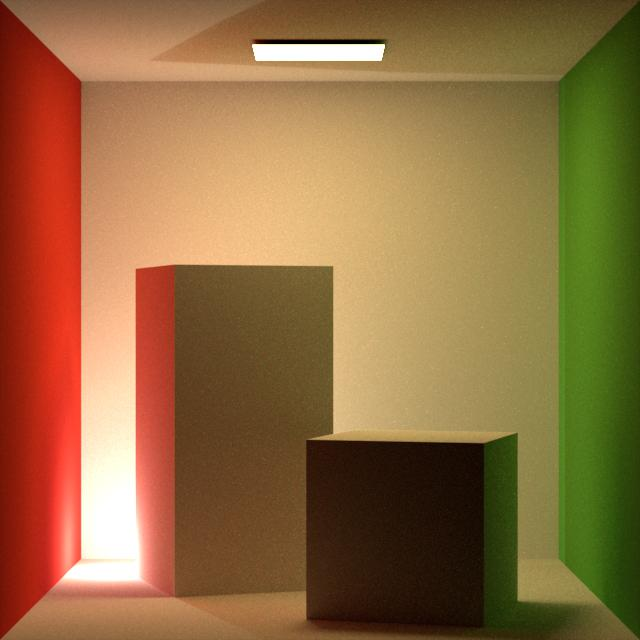
\includegraphics[width=\textwidth]{images/02-linear_lt_comb.jpg}
        \caption*{\(a = 1.0\), \(b = 1.0\)}
        %\label{}
    \end{subfigure}
    \hfill
    \begin{subfigure}[b]{0.24\textwidth}
        \centering
        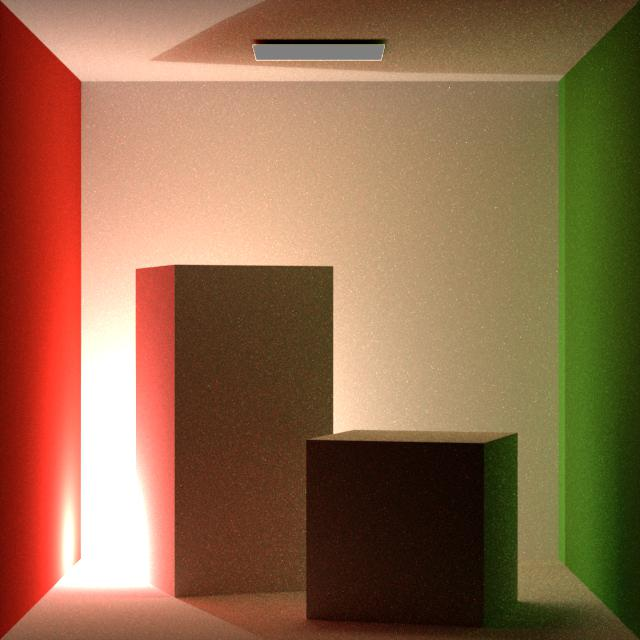
\includegraphics[width=\textwidth]{images/02-linear_lt_comb2.jpg}
        \caption*{\(a = 0.5\), \(b = 2.0\)}
        %\label{}
    \end{subfigure}
    \caption{Demonstration of the linearity of light transport. The scene displayed here has two light sources: on the ceiling and in the back corner. This means that its light transport can be captured using two basis images \(x_1\) and \(x_2\). Each of the above images was then created using a linear combination of the basis images: \(a \cdot x_1 + b \cdot x_2\)}
    \label{fig:background_linear_lt}
\end{figure}

As a consequence, radiance incoming onto a given camera sensor can be determined by the \textit{light transport (LT) matrix} \(A\):

\begin{equation}
    \label{eq:lt_matrix}
    A = \begin{bmatrix}
        c_{11} & c_{21} & c_{31} & \dots & c_{m1} \\
        c_{12} & c_{22} & c_{32} & \dots & c_{m2} \\
        c_{13} & c_{23} & c_{33} & \dots & c_{m3} \\
        \vdots & \vdots & \vdots & \ddots & \vdots \\
        c_{1n} & c_{2n} & c_{3n} & \dots & c_{mn}
    \end{bmatrix}
\end{equation}

where \(m\) is the number of light sources in a scene, \(n\) is the number of pixels in the camera sensor and \(c_{ij}\) is the value of the \(j\)-th pixel of an image that was rendered with only the \(i\)-th light source turned on. By taking a linear combination of the columns of the matrix it is then possible to obtain an image rendered by the corresponding combination of light sources.

In projection mapping, this matrix is usually extremely large because \(n\) corresponds to camera resolution and \(m\) corresponds to projector resolution. Also, in colorful images, each \(c_{ij}\) is a 3-dimensional vector. The two main challenges are therefore

\begin{itemize}
    \item Capturing the matrix
    \item Obtaining its inverse
\end{itemize}

In practice, it is impossible to capture the matrix by projecting a canonical basis because this would mean projecting with only a single pixel turned on and the signal-noise ratio of camera sensors is too high to capture such faint light. While it would be possible to project a different basis that is detectable by a camera, such a process would still be very time consuming. Methods for light transport capture usually rely on the fact that the LT matrix is often very sparse. In fact, the less inter-reflection there is in a scene, the sparser the matrix is. One example of a method that reconstructs the matrix using a limited number of samples is \citet{Peers2009}. Using that method it is possible to capture a matrix with \(m = 128^2\) using 991 measurements.

Inverting the matrix (or, more precisely, obtaining its pseudo-inverse because it is not generally square) is also practically impossible due to the size of the matrix. The solution is again to use the sparsity of the matrix to arrive at an estimate.

For example, \citet{Wetzstein2007} use the inverse light transport approach to implement a projection mapping method which works with arbitrary scenes and also compensates projector defocus which previously mentiones methods ignored. The drawbacks of this method are several hours long matrix acquisition process (during and after which the scene needs to stay static) and also the loss of some global illumination effects caused by estimates of both the LT matrix and its pseudo-inverse. Example results can be seen in fig. \ref{fig:background_wetzstein_result}.

\begin{figure}[ht]
    \centering
    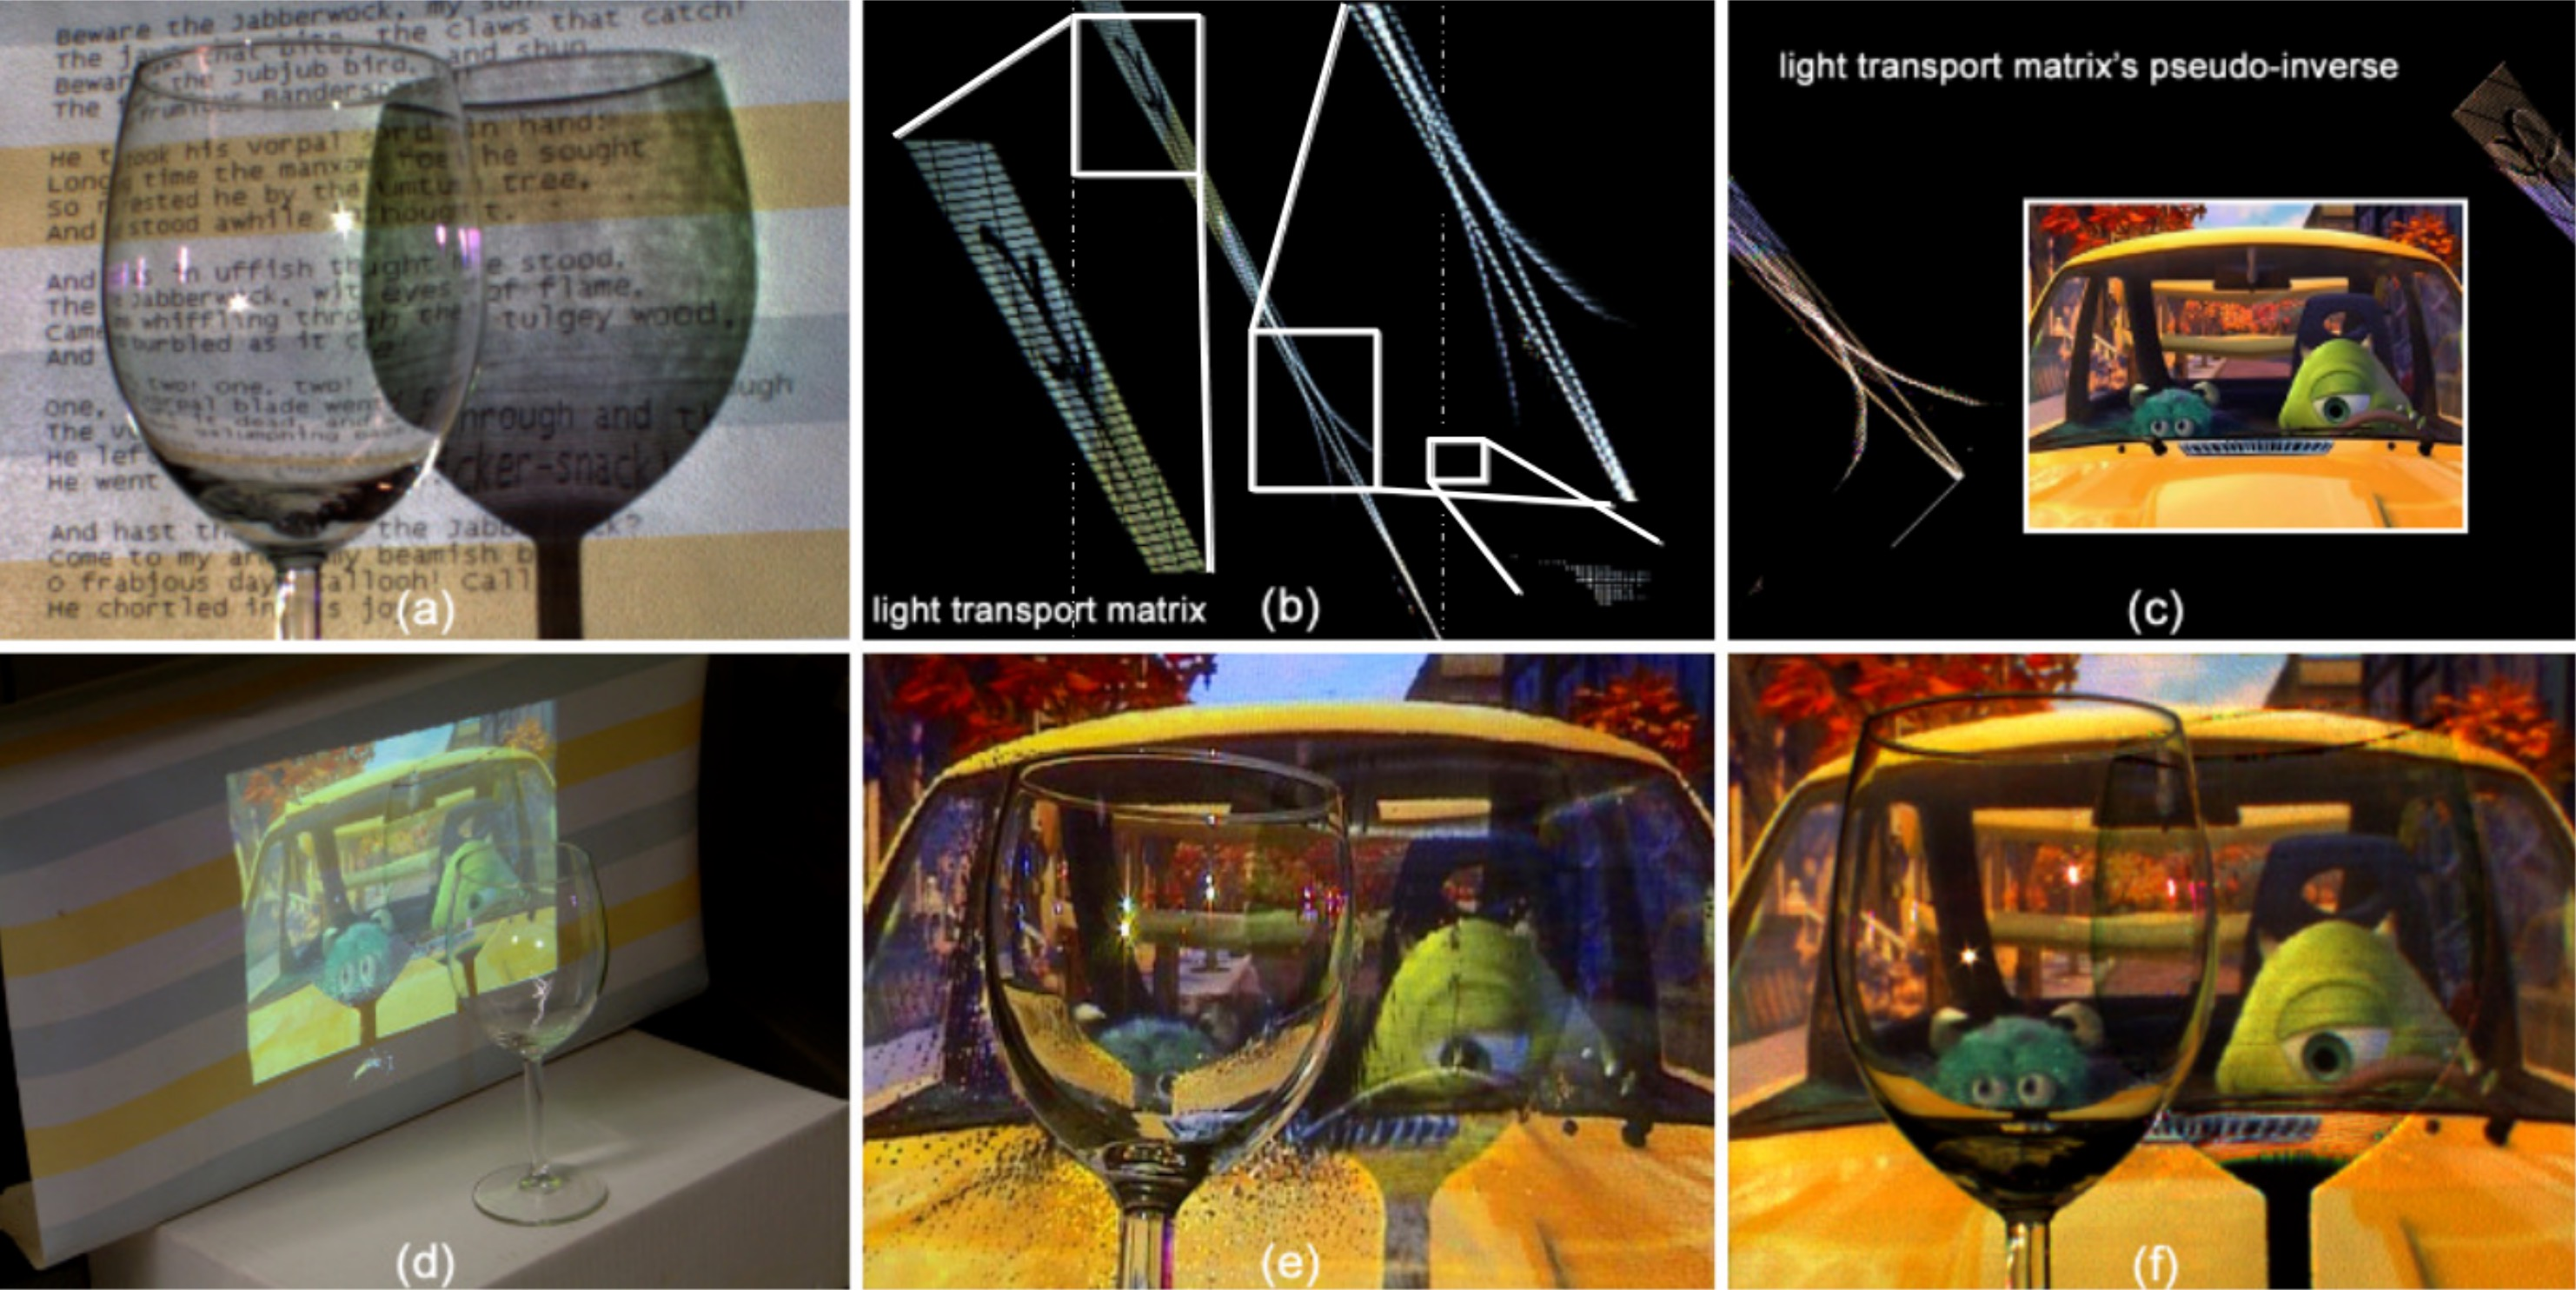
\includegraphics[width=0.8\textwidth]{images/02-wetzstein_result_compressed.jpg}
    \caption{Results of a projection mapping method by \citet{Wetzstein2007}. A wine glass in front of a colored wallpaper (a). The light transport matrix’s (b) pseudo-inverse (c, background) is approximated with a clustering scheme and allows a real-time compensation for displaying interactive content and movies (c) - from an angle (d), compensated with a conventional method (e) and with inverse light transport (f). Source: \citet{Wetzstein2007}}
    \label{fig:background_wetzstein_result}
\end{figure}

This concludes the section on projection mapping which was aiming to explain how to predict what an image will look like when projected onto a scene. We now move on to the second topic that our method builds on. This time we focus on what a texture is and how to generate new realizations of a given texture sample.

\section{Texture Synthesis}
\label{section:background-texture_synthesis}

As mentioned in section \ref{section:intro-key_idea}, the aim of this thesis is to advance the idea of content-based projection mapping of textures. As section \ref{section:background-projection_mapping} suggests, with current projector hardware it is not always possible to match the camera image with the desired appearance pixel by pixel while minimizing clipping errors. Hence in our method we loosen up the definition of image similarity. Textures are a great candidate for that because two textures can have radically different pixel values in corresponding position but still look the same (see fig. \ref{fig:background_similar_textures} for an example).

\begin{figure}[ht]
    \centering
    \begin{subfigure}[b]{0.48\textwidth}
        \centering
        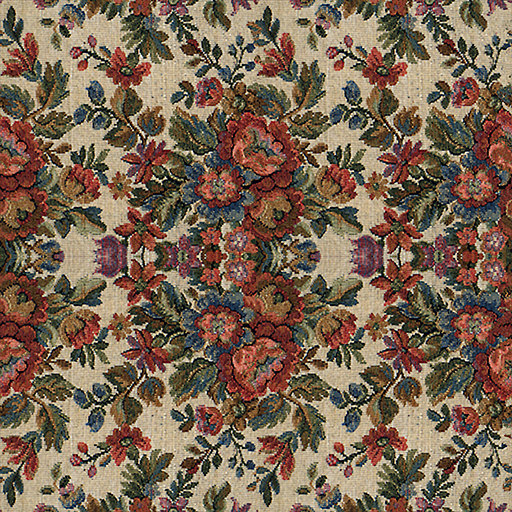
\includegraphics[width=\textwidth]{images/02-flowers1.png}
        \caption*{}
        %\label{}
    \end{subfigure}
    \hfill
    \begin{subfigure}[b]{0.48\textwidth}
        \centering
        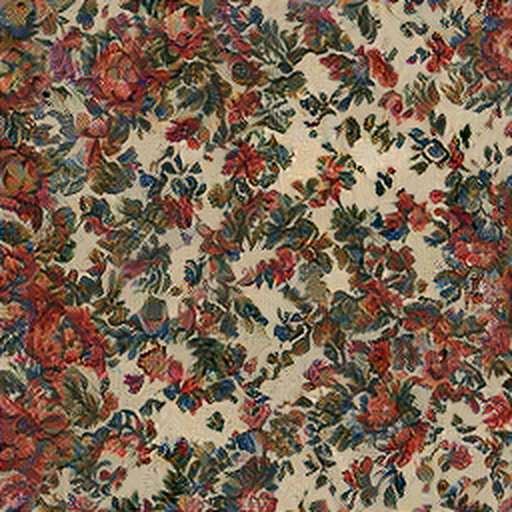
\includegraphics[width=\textwidth]{images/02-flowers2.png}
        \caption*{}
        %\label{}
    \end{subfigure}
    \caption{An example of two realizations of the same texture. The image on the right was created by a texture synthesis method by \citet{Gatys2015}. Texture source: \citet{Pixar128}, modified}
    \label{fig:background_similar_textures}
\end{figure}

But what exactly is a texture and what kind of image modifications can be done while preserving it? In this section, we provide an overview of texture synthesis research which is the second building block that our method relies on.

\subsection{Textures}
\label{section:background-texture_synthesis-textures}

Figures \ref{fig:intro_pixels_vs_stats} and \ref{fig:background_similar_textures} show examples of textures. Unfortunately, according to \citet{Raad2018} there is no universally accepted mathematical definition of what constitues a texture. Researchers who have attempted to characterize textures have usually defined them in terms of human vision. For example, \citet{Julesz1962}, one of the most prominent researchers in this field has defined textures as classes of images that cannot be discriminated in preattantive (i.e. effortless or instantaneous) vision and then attempted to characterize them mathematically.

How should then one go about doing texture synthesis (i.e. generating new examples of a given texture class) when there is no formal definition of what a texture is? Existing methods can be divided into two categories based on how they approach this problem:

\begin{enumerate}
    \item Find a new candidate for texture definition which forms a texture model and then generate images according to that model. This category is also called \textit{parametric texture synthesis} or \textit{statistics-based texture synthesis} (because the model is usually a statistical one)
    \item Work without a model and instead define a procedure that turns one texture example into a new one. This category is also called \textit{non-parametric texture synthesis} or \textit{patch-based texture synthesis} (because the procedure usually operates on patches of the texture image)
\end{enumerate}

In the following sections we explain the theoretical background of both approaches to texture synthesis and describe the most important methods in each category. Specifically, we focus on strengths and weaknesses of each method and on how suitable it is for our purpose of projection mapping of textures as outlined in section \ref{section:intro-key_idea}. For a more in-depth review of the state of the art in texture synthesis, see \citet{Raad2018}.

\subsection{Patch-Based Texture Synthesis}
\label{section:background-texture_synthesis-patch_based}

We begin with patch-based texture synthesis because it is conceptually simpler and achieves very good results for particular kind of textures. The basic idea was introduced by \citet{Efros1999} and was inspired by \citet{Shannon1948} and his use of a Markov chain to generate English text. Here is an example of Shannon's method (taken from \citet{Raad2018}):

\begin{itemize}
    \item in no ist lat whey cratict froure birs grocid pondenome of demonstures of the reptagin is regoactiona of cre
\end{itemize}

Analogously to two different texture realizations, this sentence is not English, but looks like it. It is generated letter by letter by sampling from a probability distribution of an English text sample conditioned on the previous \(n = 3\) letters.

In their texture synthesis method, \citet{Efros1999} generate an image pixel by pixel based on a probability distribution of the given texture sample. We will desribe how exactly this method works on an improved version of it, called \textit{image quilting}, which was introduced by \citet{Efros2001}.

\subsubsection{Image Quilting}
\label{section:background-texture_synthesis-patch_based-quilting}

\begin{figure}[ht]
    \centering
    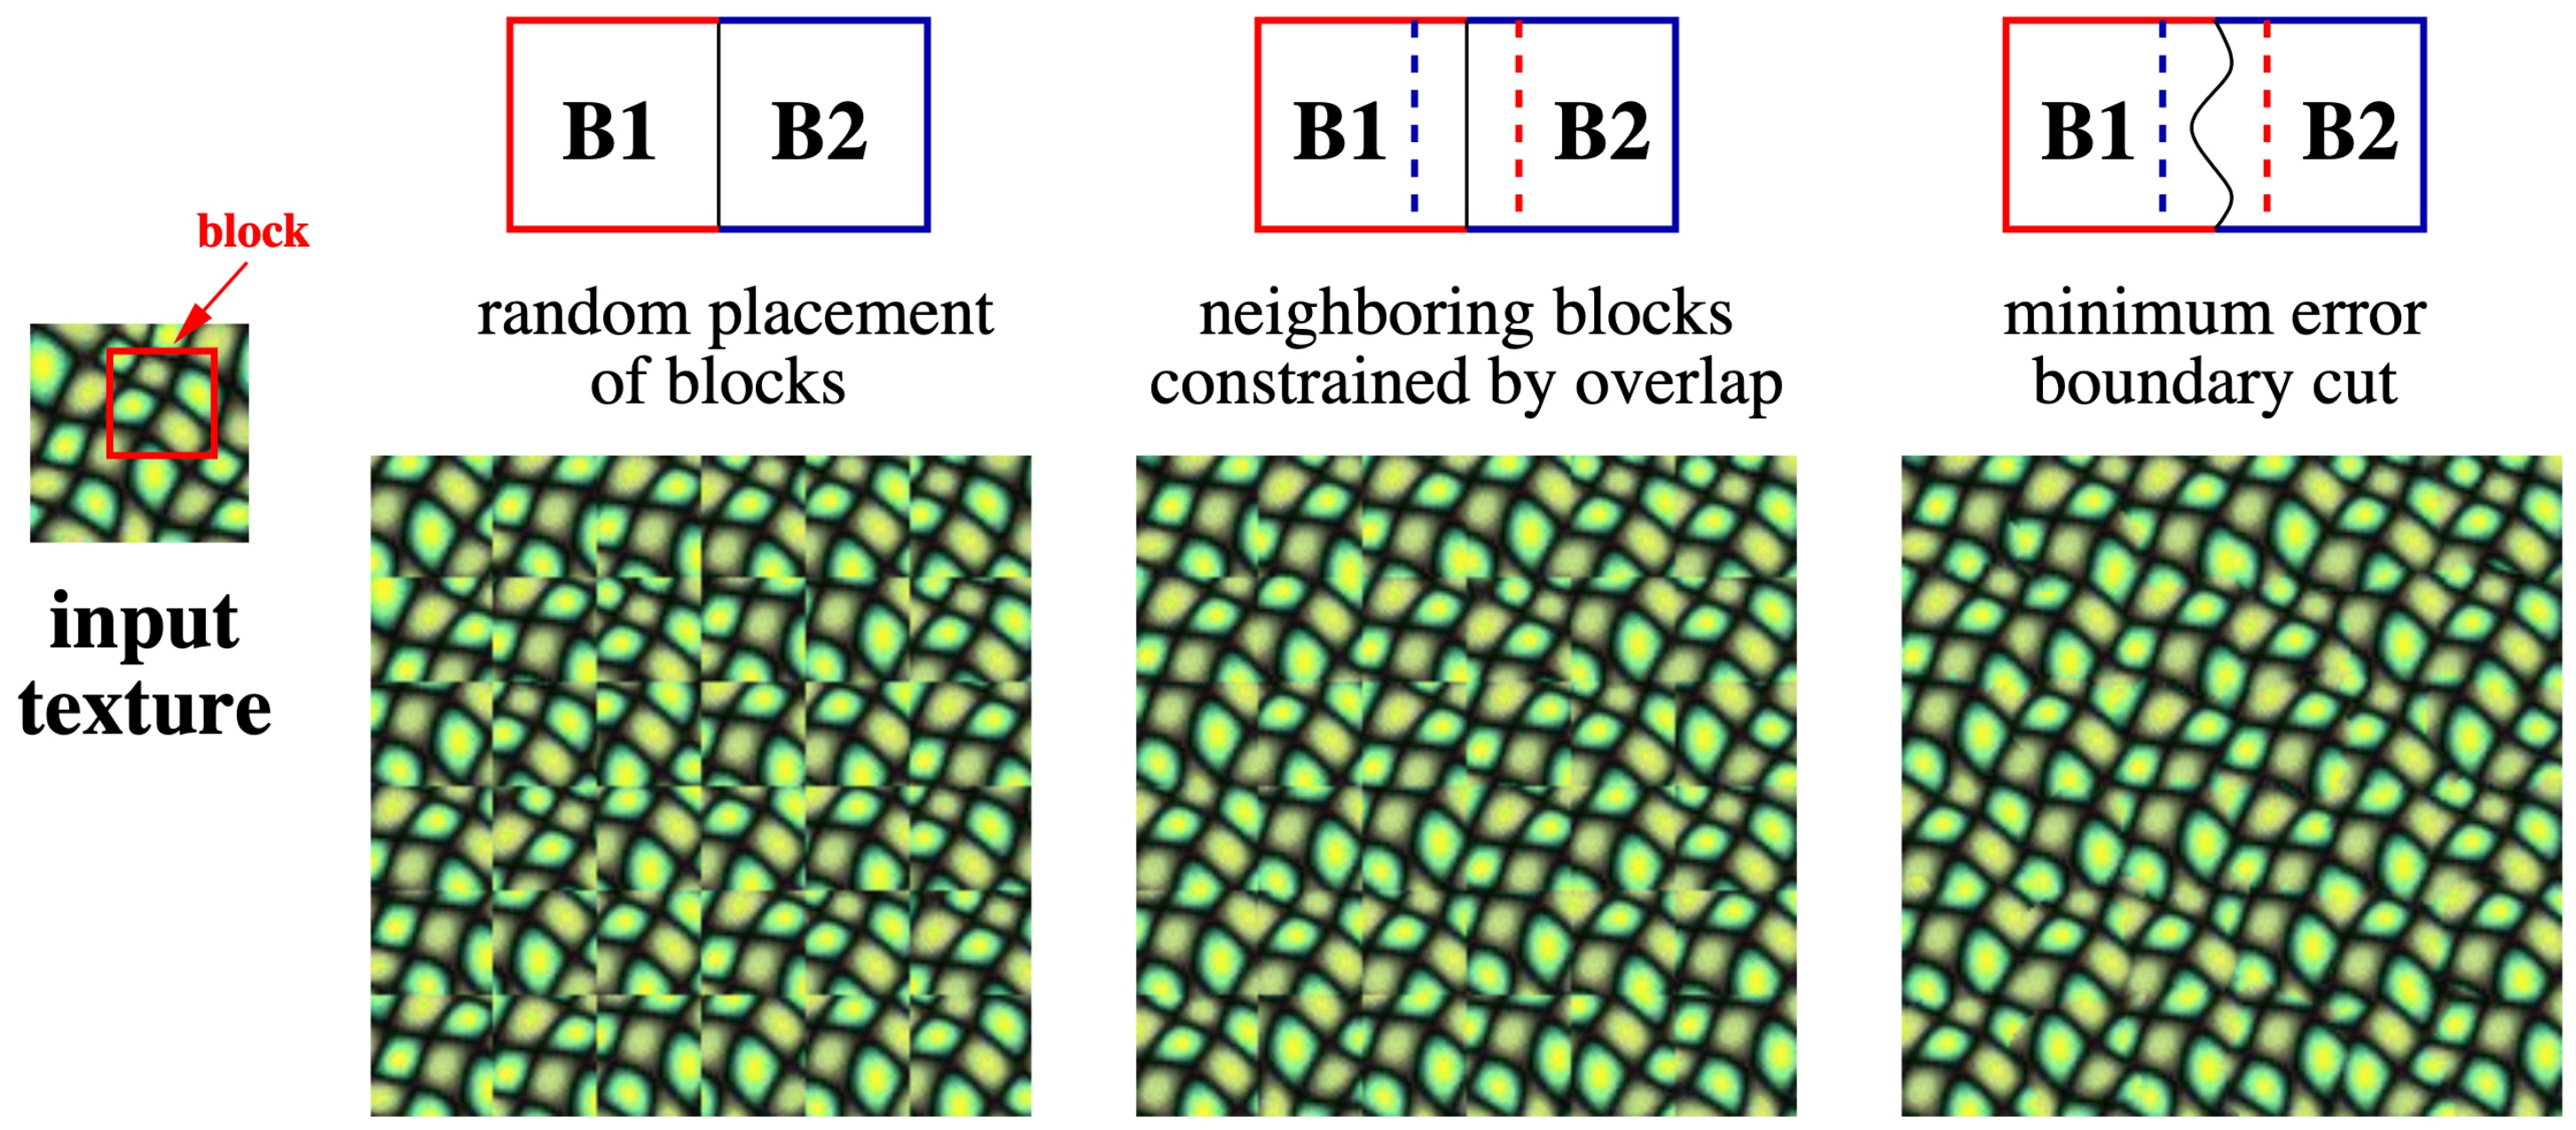
\includegraphics[width=\textwidth]{images/02-quilting_method_compressed.jpg}
    \caption{Illustration of image quilting. The leftmost image was generated by choosing block \(B_i\) at random. The middle image was generated by choosing a block with low pixel-wise error in an overlap with the previous block. The rightmost image was generated by choosing blocks as in the middle, only the new block is pasted along a minimum error path instead of a straight line.  Source: \citet{Efros2001}}
    \label{fig:background_quilting_method}
\end{figure}

Image quilting starts by splitting the input texture image into overlapping square blocks \(B_i\) of size \(k\) (a user-controlled parameter). Then it builds a new texture block by block in raster scan order (from the top left corner to the bottom right corner, row by row). A new block \(B^{\prime}\) is chosen at random from all \(B_i\) such that the pixel-wise error in overlapping areas (they use 1/6 of block area along the edge) with the block above \(B^{\prime}\) and to the left of \(B^{\prime}\) in below a certain threshold in the output image. Since many blocks usually satisfy this overlap constraint, one is picked at random. If \(B^{\prime}\) was pasted into the output image directly, the result would look blocky. Therefore \(B^{\prime}\) is pasted into the output image along a minimum error path inside the overlapping areas. This ensures that seams between block will be as subtle as possible. See fig. \ref{fig:background_quilting_method} for an illustration of the method.

\subsubsection{Pros and Cons}
\label{section:background-texture_synthesis-patch_based-pros_and_cons}

This method can achieve stunning visual results when the input texture is uniformly lit and contains large features, like pebbles or coffee beans. It is especially powerful when used on textures with regular structure, like a brick wall. See fig. \ref{fig:background_quilting_pros_cons} for an example.

However, it struggles with textures that have non-uniform illumination and that contain very small features, like sand or concrete. Failure cases usually manifest themselves by large areas that are directly copied from the input (so-called \textit{verbatim copying}) or areas that contain the same patch copied over and over (so-called \textit{garbage growing}). See fig. \ref{fig:background_quilting_pros_cons} for an example.

\begin{figure}[ht]
    \centering
    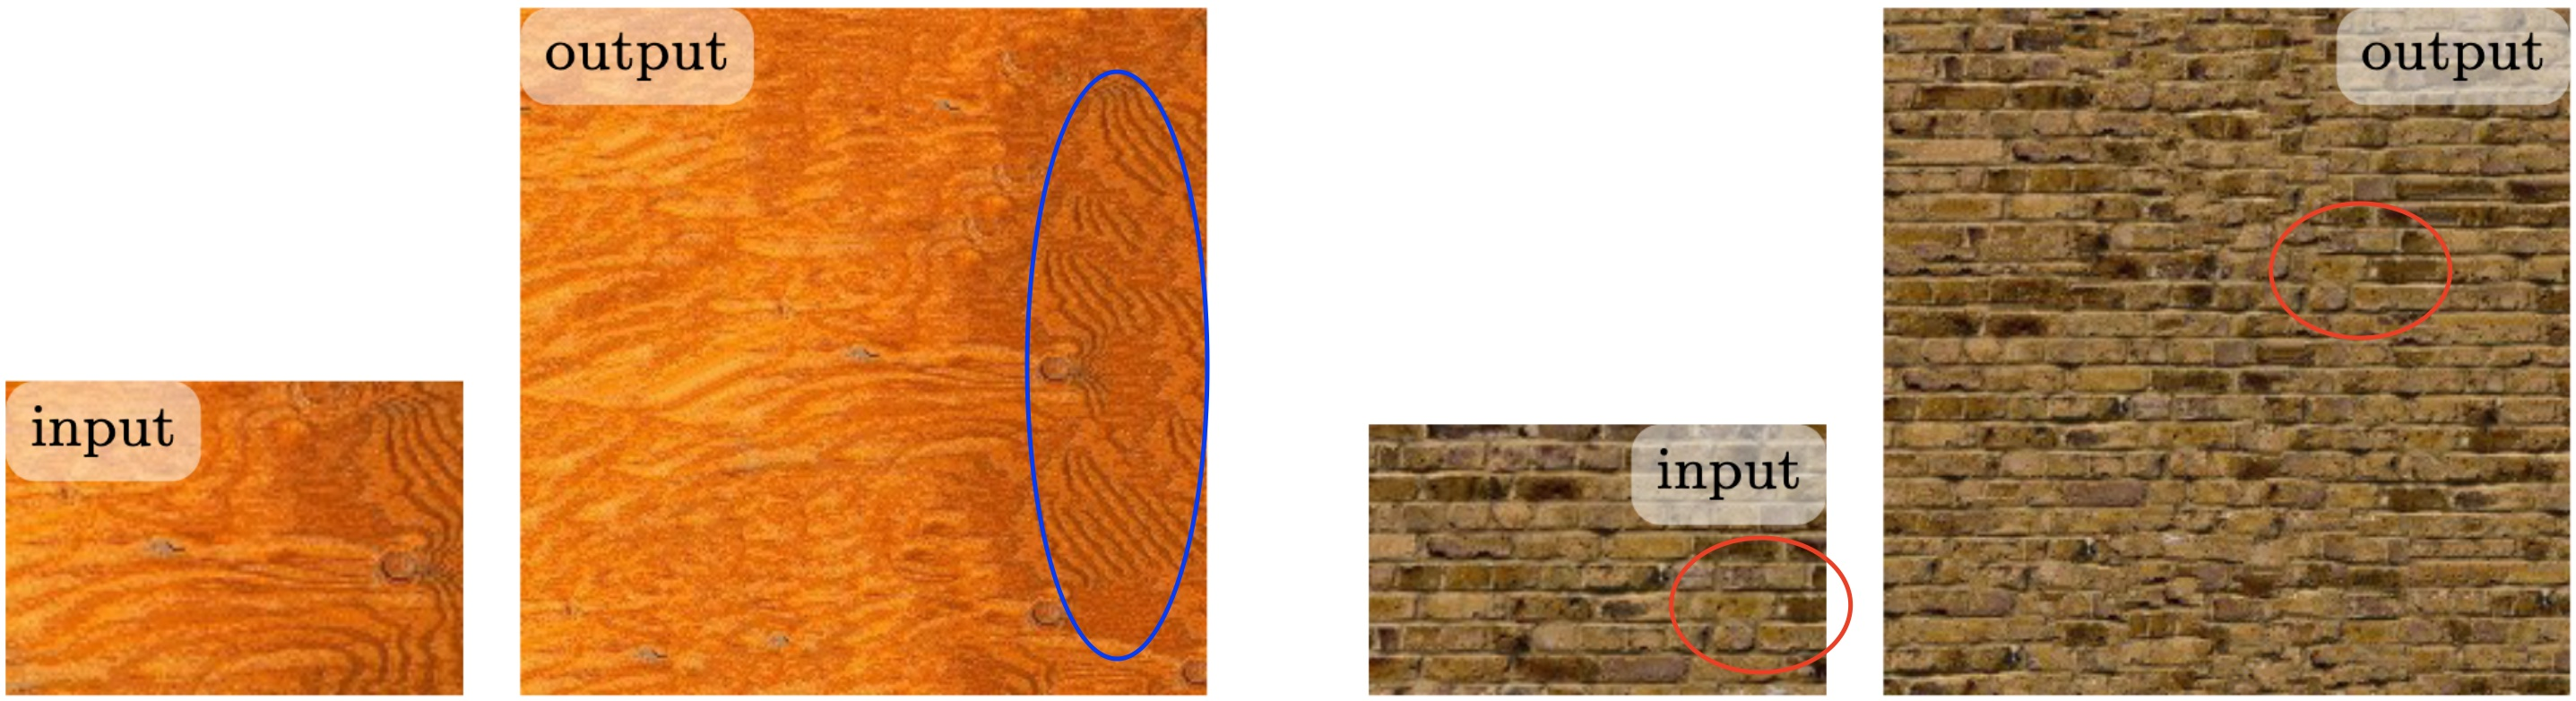
\includegraphics[width=\textwidth]{images/02-quilting_pros_cons_compressed.jpg}
    \caption{Examples of image quilting. On the left is a failure with the garbage growing effect highlighted in blue. On the right is a success. However, some verbatim copies (highlighted in red) are clearly visible in the rightmost image. Source: \citet{Raad2018}, highlighting own}
    \label{fig:background_quilting_pros_cons}
\end{figure}

Another drawback of this method is that its parameters need to be manually tuned based on the feature sizes and other properties of the input texture. There is also no underlying texture model that this method would work with which means that reasoning about it is somewhat less robust and limited to measuring heuristics such as the amount of verbatim copies and garbage in the output.

\subsubsection{Potential Usage in Projection Mapping}
\label{section:background-texture_synthesis-patch_based-projection_mapping}

Image quilting is surprisingly flexible to adapt for other uses than texture synthesis. The authors themselves showcase the possibility of using the method for style transfer. This is a problem that considers two input images and produces a third one which has the content of one image and style of the other. This can be achieved by adding a new term to the overlap error. In the case of style transfer, it takes the form of the difference in pixel intensities of the candidate patch and a corresponding patch of the target image. See fig. \ref{fig:background_quilting_transfer} for an example.

\begin{figure}[ht]
    \centering
    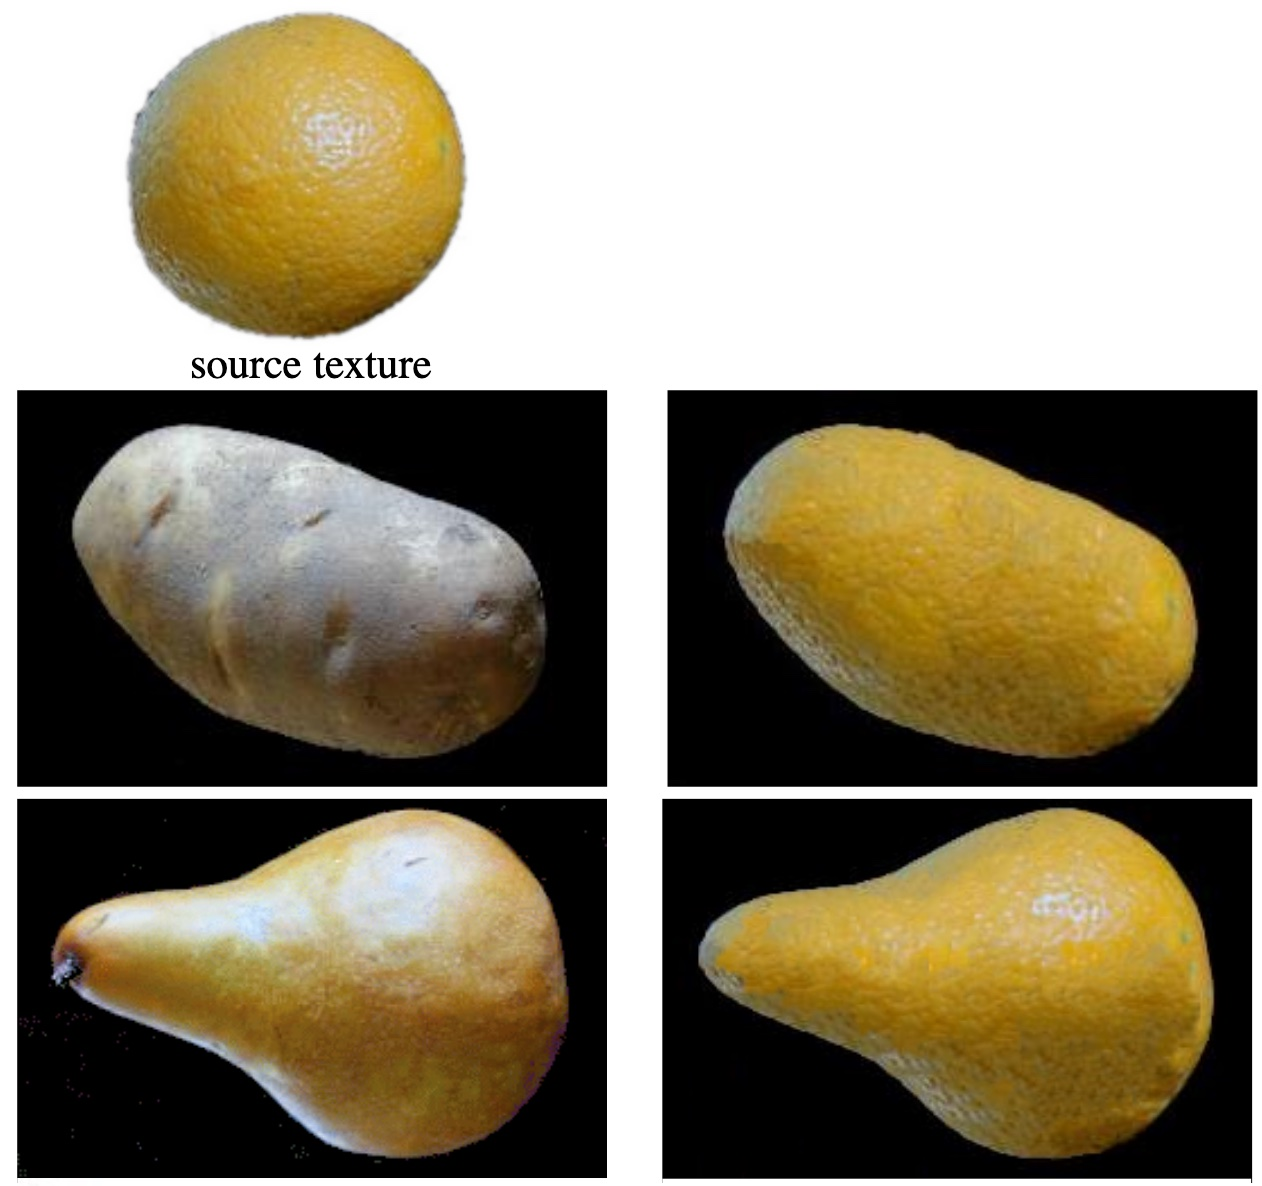
\includegraphics[width=0.6\textwidth]{images/02-quilting_transfer_compressed.jpg}
    \caption{Example of style transfer using image quilting. The output (right) is generated just like during texture synthesis except for two changes: 1) the output image size is chosen to be that of the target image (left) and 2) an extra term is added to the overlap error. This term represents the difference between the pixel intensities of the candidate patch and a corresponding patch of the target image. Source: \citet{Efros2001}}
    \label{fig:background_quilting_transfer}
\end{figure}

One could imagine using this method for projection mapping by modifying the overlap error term. Roughly speaking, the additional error term could be proportional to how difficult it would be to radiometrically compensate the candidate patch. More specifically, the candiate patch would first be radiometrically compensated and then the error would be set to the inverse distance of the compensation and the limit of the projector gamut. This could be built on top of methods such as \citet{Grundhofer2015} that assume 1:1 correspondence between projector image and camera image.

\subsection{Statistics-Based Texture Synthesis}
\label{section:background-texture_synthesis-statistics_based}

{\color{red} TODO: mention the Texture Hypothesis by Julesz (texture is defined by 2nd order co-occuring stationary statistics) here}

{\color{red} TODO: provide the deeper theory that used to be in the intro, but isn't anymore}

All statistics-based methods for texture synthesis share the general workflow. They first extract a set of statistics from the input texture image. Then they initialize a random noise image and iteratively optimize it so that its statistics are the same as those of the input image ({\color{red} TODO: figure}). Different initializations of the noise image yield different final results (unless the statistics are too restrictive so as to represent only one image) and by computing the difference between the statistics of the input and the output we can easily argue about convergence of such methods.

\citet{Gatys2015} have introduced a breakthrough method for statistics-based texture synthesis which significantly improved over the previous state of the art. This method relies on a \textit{convolutional neural network} (CNN) to produce a statistical description of a texture image that the noise initialization is then optimized to fit. Let us first briefly introduce what a CNN and what makes it so powerful at creating abstract descriptions of images.

\subsubsection{Convolutional Neural Networks (CNNs)}
\label{section:background-texture_synthesis-statistics_based-cnns}

\textit{Neural networks}, or more precisely \textit{feedforward neural networks}, are essentially functions

\begin{equation}
    \label{eq:neural_network}
    y = f(x, \phi)
\end{equation}

where \(x\) is the input, \(y\) is the output and \(\phi\) are the parameters of a neural network. The idea is that \(f\) is an approximation of \(f^\star\) which is a very complex, non-linear function which tells us something about the world. For example, we can consider \(f^\star\) to be the mapping between all possible images of size \(224 \times 224\) and categories such as dog, cat, tree, house, etc. that describe the image. The goal of \textit{deep learning}, which is the study of feedforward and other kinds of neural networks, is then to find an \(f\) along with its parameters \(\phi\) that approximate \(f^\star\) as closely as possible. Because of the complexity of \(f^\star\), \(f(x) = f^{(3)}(f^{(2)}(f^{(1})(x)))\) is often composed of many functions \(f^{(i)}\) which are called \textit{layers}. Each layer usually operates on vectors and is commposed of small units that are loosely modeled on brain neurons. Together, these layers form a network where information flows from the first layer to the last. Hence the term \textit{feedforward neural network}.

{\color{red} TODO: mention training?}

Convolutional neural networks (CNNs) form a class of neural networks that are intended for processing grid-like inputs, for example images (2D grid) or audio (1D grid). Their layers are typically composed of three parts: convolution, nonlinearity and pooling.

{\color{red} TODO: image}

\textbf{Convolution}. To explain convolution in the context of neural networks, it is best to start with an example. Let us imagine that we have an image and would like to find all vertical edges in that image. This can be done using convolution ({\color{red} TODO: image}). All we need to do is take a \(3 \times 3\) matrix ({\color{red} TODO: figure out the right values\dots}), also called \(kernel\), move it across the image aligning the center of the kernel with each image pixel in turn, multiplying overlapping values, summing them together and writing them out into a new image. We will notice that the new image contains high values in places where there is a vertical edge in the original image. What has happened?

The process we have gone through with our image and our kernel is called convolution in the context of deep learning, although strictly speaking, it corresponds to cross-correlation which differs from convolution by the orientation of the kernel. Our kernel happens have values which detect vertical edges when convolved with an image. Kernels with different values do different things, for example detect horizontal edges, blur the image, or even leave it untouched ({\color{red} TODO: examples!}).

Kernel values are what constitutes the parameters \(\phi\) of a CNN and it turns out that they are powerful enough to achieve impressive results in tasks such as object recognition, ({\color{red} TODO: more examples}). They cannot function alone, however. As we have mentioned, neural networks usually approximate complex non-linear function and convolutions as presented here are linear. Two more building blocks are therefore needed.

\textbf{Nonlinearity}. Nonlinearities are scalar functions whose purpose is to simply introduce nonlinear behavior into a CNN. Many types of nonlinearities have been proposed in recent years, for example hyperbolic tangent or ReLU ({\color{red} TODO: figures}). ReLU is used more commonly simply because it improves results ({\color{red} TODO: maybe cite some justification for this?}).

\textbf{Pooling}. Pooling functions are function that accept a vector as input and return a scalar as output. They are often use to make CNNs invariant to small shifts in the input image and also reduce the size of the intermediate outputs, also called \textit{activations}, of each CNN layer. ({\color{red} TODO: a bit more explanation with images?})

CNNs typically have multiple such layers and since they are trained to classify images, the have a few fully connected layers ({\color{red} TODO:  explain?}) at the end which compress the activations into an \(n\)-dimensional vector where each position of the vector corresponds to a particular image class and the value at that position tells how likely the input image is to belong to that image class. For a more comprehensive overview of neural networks and deep learning, see \citet{Goodfellow2016}. We will now focus how CNNs are related to texture synthesis.

{\color{red} TODO: depth of output? number of feature maps? RGB channels?}

{\color{red} TODO: biases?}

{\color{red} TODO: fully connected layers? classification output?}

For texture synthesis as introduced by \citet{Gatys2015}, however, it is only the activations after individual convolution layers that matter. The operation of convolution and the fact that the network is trained to classify images ({\color{red} TODO: deep image prior?}) causes those activations to contain filtered versions of the input image where particular features that define a texture are emphasized ({\color{red} TODO: now it would be great to have a visualization of which features are picked out at which levels!}).

\subsubsection{Texture Synthesis Using CNNs}
\label{section:background-texture_synthesis-statistics_based-synthesis_using_cnns}

As mentioned in \ref{section:background-texture_synthesis-statistics_based}, statistics-based texture synthesis relies on a statistical description of a texture that white noise images are optimized to match. \citet{Gatys2015} use the activations after each pooling layer of the VGG-19 CNN by \citet{Simonyan2014} to define such a description. These activations, however, contain spatial information of where each feature is located in the texture. In order to remove this spatial information, activation are correlated with each other within each layer. Correlated per-layer activations of VGG-19 therefore constitute a set of statistics completely describing a texture.

To synthesize a new example of a given texture, gradient-based loss optimization is used. The loss is defined as a weighted mean square error between the description of the input texture and the image being optimized. The L-BFGS optimizer is used to drive the optimization process ({\color{red} TODO: why is it a good choice?}).

Let us now summarize exactly what constitutes a texture model in \citet{Gatys2015}.

{\color{red} TODO: give the details to be complete. or leave them for appendix?}

\subsubsection{Pros and Cons}
\label{section:background-texture_synthesis-statistics_based-pros_and_cons}

{\color{red} TODO: show some examples from the paper where they compare to Portilla and Simoncelli}

{\color{red} TODO: refer to \citet{Raad2018} for some more pros and cons\dots}

This method of synthesizing textures leads to high-quality results for a large variety of input images. Compared to patch-based synthesis it also provides a texture model, as opposed to a mere algorithm to generate new textures. This makes it easier to reason about and provide theoretical justifications as to why it works.

One disadvantage of this method is that it struggles with regular patterns, unline patch-based methods. It is also fairly sensitive to input and output image resolution {\color{red} TODO: explain this properly}

\subsubsection{Potential Usage in Projection Mapping}
\label{section:background-texture_synthesis-statistics_based-projection_mapping}

This method could be easily adapted to projection mapping if a differentiable rendering function was added to the optimization loop. The idea is to first project initial white noise image onto a scene and then feed the resulting camera image into the CNN and ultimately compare it against the input texture image. The loss gradients would flow through both the CNN and the rendering function and would be used to update the initial image. The result of this process should be an image which once projected looks like a new example of the input texture.